% !TeX root = ./thesis.tex










%==============================
\chapter[A balanced mixture of antagonistic pressures promotes\\ the evolution of parallel movement]{A balanced mixture of antagonistic pressures\\ promotes the evolution of\\ parallel movement}
\chaptermark{A balanced mixture of antagonistic pressures promotes parallel movement} % change running head for chapter
\label{chap:scirep}

\chapterAbstract[published={scirep/Demšar_etal_2016.pdf}, keywords={Collective behaviour, evolution, fuzzy logic, predator-prey interaction, dynamic parallel group}]{A common hypothesis about the origins of collective behaviour suggests that animals might live and move in groups to increase their chances of surviving predator attacks. This hypothesis is supported by several studies that use computational models to simulate natural evolution. These studies, however, either tune an ad-hoc model to ``reproduce'' collective behaviour, or concentrate on a single type of predation pressure, or infer the emergence of collective behaviour from an increase in prey density. In nature, prey are often targeted by multiple predator species simultaneously and this might have played a pivotal role in the evolution of collective behaviour. We expand on previous research by using an evolutionary rule-based system to simulate the evolution of prey behaviour when prey are subject to multiple simultaneous predation pressures. We analyse the evolved behaviour via prey density, polarization, and angular momentum. Our results suggest that a mixture of antagonistic external pressures that simultaneously steer prey towards grouping and dispersing might be required for prey individuals to evolve dynamic parallel movement.}

%-----
\section{Introduction}

Results from studies of collective behaviour are useful for scientists from many different research fields -- from biology, physics and medicine, to computer science \cite{deisboeck2009collective,lebarbajec2009organized,sumpter2006principles,vicsek1995novel,xu2014crowd}. Because humans behave similarly as groups of animals in a wide repertoire of situations, such as traffic jams and behaviour at large-scale events (\eg sport games, music concerts), collective behaviour is also interesting from the social studies perspective \cite{sumpter2006principles,xu2014crowd}.

The literature about collective behaviour contains several hypotheses about why animals, such as schools of fish, flocks of birds, swarms of insects, and herds of ungulates coalesce into groups. Some studies suggest that animal groups may increase the mating and foraging efficiency of their members \cite{krebs1994behavioural}, or that grouping could save energy because of hydrodynamic or aerodynamic benefits \cite{hemelrijk2014increased,marras2015fish,portugal2014upwash}.

Probably the most common hypotheses about the evolution of collective behaviour are related to protection from predation \cite{cresswell2011predicting,hart2005predator,krause2002living,larsson2012why,lebarbajec2009organized,nishimura2002predator,pavlov2000patterns}. The selfish herd hypothesis suggests that animals form groups in order to reduce their individual domain of danger \cite{hamilton1971geometry,kimbell2015selfish,morrell2015consequences}. The confusion effect hypothesis states that a predator attacking a group of visually similar prey might have a hard time tracking and capturing its target \cite{demsar2015simulating,kunz2006prey,nishimura2002predator,olson2013predator,olson2016evolution,zheng2005behavior}. The many eyes hypothesis suggests that as the size of the group increases the amount of time an individual has to scan the environment decreases \cite{haley2014exploring,ruxton2008application}. And the dilution of risk hypothesis suggests that the chance of a single prey being selected as the predator's target is lower in larger groups \cite{tosh2011conditions}.

Computational models are becoming a frequent tool for studying various hypotheses concerning collective behaviour \cite{lebarbajec2009organized,sumpter2006principles,vicsek2012collective}. In computational models genetic algorithms \cite{holland1992adaptation} and genetic programming \cite{koza1992genetic} are usually used to simulate artificial evolution. Artificial evolution can help us understand which selective pressures may have been the reason for collective behaviour to evolve. Wood \& Ackland \cite{wood2007evolving} used genetic algorithms to tune parameters of the model that was originally presented by Couzin\etal \cite{couzin2002collective} to suggest that predation might promote the evolution of laterally expanded visual perception. Kunz\etal \cite{kunz2006prey} evolved artificial neural networks to show that the presence of a confusable predator might be a sufficient condition for prey individuals to evolve collective behaviour. Using a comparable technique, a similar result was achieved by Olson\etal \cite{olson2013predator,olson2016evolution}, who in addition showed that predators may reduce the benefits of prey grouping by attacking peripheral targets and that grouping evolves when the predators attack prey individuals that are located nearby. Morrell\etal \cite{morrell2015consequences} showed that complex rules outperform simple ones under a range of predator attack strategies. As a contrast Demšar\etal \cite{demsar2015simulating} used genetic algorithms to evolve composite predation tactics and showed that confusion might play an important role in the evolution of these. A recent study by Biswas\etal \cite{biswas2014causes} suggests that the dilution of risk is the most prominent factor for the evolution of clumping and not the confusion effect as suggested by previous research. 

In the studies that investigated the evolution of collective behaviour under various predation tactics \cite{biswas2014causes,morrell2015consequences,olson2013predator,olson2016evolution} researchers were mostly interested in whether prey individuals start to group or not (\ie whether as a result of the artificial evolution the prey density increased or decreased). As groups of animals in nature move in many different regimes (clumping, swarming, milling, schooling, etc.) \cite{krause2002living,suzuki1973movement} and different predation pressures are countered by different responses of prey groups, we can hypothesise that the type of predation tactic has an influence on the type of collective behaviour that evolves.

In this study we focus on how predation from various types of predators influences the evolution of collective behaviour in prey individuals. We let prey individuals evolve their behaviour while experiencing predation from a) predators for which grouping might be a natural response and b) predators for which dispersing might be a natural response. According to previous research there are several predation tactics that pressure prey individuals to evolve grouping behaviour \cite{biswas2014causes,kunz2006prey,olson2013predator,olson2016evolution}. Two of these are a) attack prey individuals located at the periphery of the prey group (P, periphery) and b) attack the nearest prey individual (N, nearest). Predation tactics that pressure prey towards dispersing (against grouping behaviour), are a) attack the most central prey individual in a prey group (C, centre) and b) high density area attacks (H, density) \cite{olson2013predator}. 

Predators that attack the nearest, the most peripheral or the most central prey individual usually detect, pursue, attack and capture a single prey individual. For example, black seabass, \emph{Centropristis striata}, in attacks on schools of Atlantic silversides, \emph{Menidia menidia}, focus on stragglers when these are available, otherwise they most often target central prey \cite{parrish1989reexamining}. Predators that focus on nearest prey individuals are typically sit-and-wait, ambush or surprise-attack predators (\eg largemouth bass, \emph{Micropterus salmoides} \cite{savino1982predatorprey} or peregrine falcons, \emph{Falco peregrinus} \cite{zoratto2010aerial}) who try to minimize energy costs required for prey capture. However, rather than relying on a single predation tactic predators usually adapt their tactic with respect to the prey species. For example, in attacks on either free-swimming whirligig beetles, \emph{Dineutes discolor}, or a constrained group of tadpoles, \emph{Bufo bufo}, largemouth bass, \emph{Micropterous salmoides}, like goldfish, \emph{Carassius auratus}, preferentially attack prey on the periphery \cite{romey2008predators}. Recent research by Ioannou\etal \cite{ioannou2012predatory} showed that bluegill sunfish, \emph{Lepomis macrochirus}, when hunting virtual prey disproportionately more often attack prey relatively far from the group centre, but only in the case when prey individuals are moving with relatively low tortuosity. In attacks on groups, on the other hand, prey in groups with a coordinated direction of motion (\ie, with high polarization) were at less risk than their counterparts in unpolarized swarms.

Density attacking predators are usually larger than a single prey individual and do not necessarily detect, pursue, attack and capture a single prey individual, but can attack and capture several prey individuals in a single predation event (\eg whales). Minke whales, \emph{Balaenoptera acutorostrata}, lunge feed on small schooling fish \cite{hoelzel1989foraging}. Killer whales, \emph{Orcinus orca}, are known to use cooperative hunting \cite{domenici2000killer,nottestad1999herring}. Basking sharks, \emph{Cetorhinus maximus}, on the other hand, are filter-feeders and feed while cruising at a relatively low and constant speed \cite{sims2000filterfeeding}. In these cases, while the prey may be able to accelerate and manoeuvre at a higher rate than the predator, the difference in size is such that, once the prey is aimed at, its speed is too low to avoid the predator's large gape \cite{domenici2001scaling}. In nature, prey living in groups are often targeted by such predators \cite{domenici2001scaling,goldbogen2011mechanics,nottestad1999herring,nottestad2002whales}, and scenarios where prey are subject to multiple predation tactics simultaneously (\eg attack single peripheral prey individuals, and density attacks) are not uncommon (\eg multi-species feedings) \cite{haynes2013molecular,mori2006first,thiebault2015howto}. Exposure to such conflicting, antagonistic predation pressures might have played a pivotal role in the evolution of collective behaviour. For this reason we investigated the type of evolved behaviour when varying exposure to multiple (conforming and antagonistic) simultaneous predation pressures.

\section{Results}

The influence of predation pressures on the evolution of prey behaviour was studied by varying the number of predators using different specific predation tactics. The total number of predators used to obtain results reported in this study was eight, but no significant difference was observed while performing preliminary tests with larger or smaller numbers of predators.

\begin{figure}
	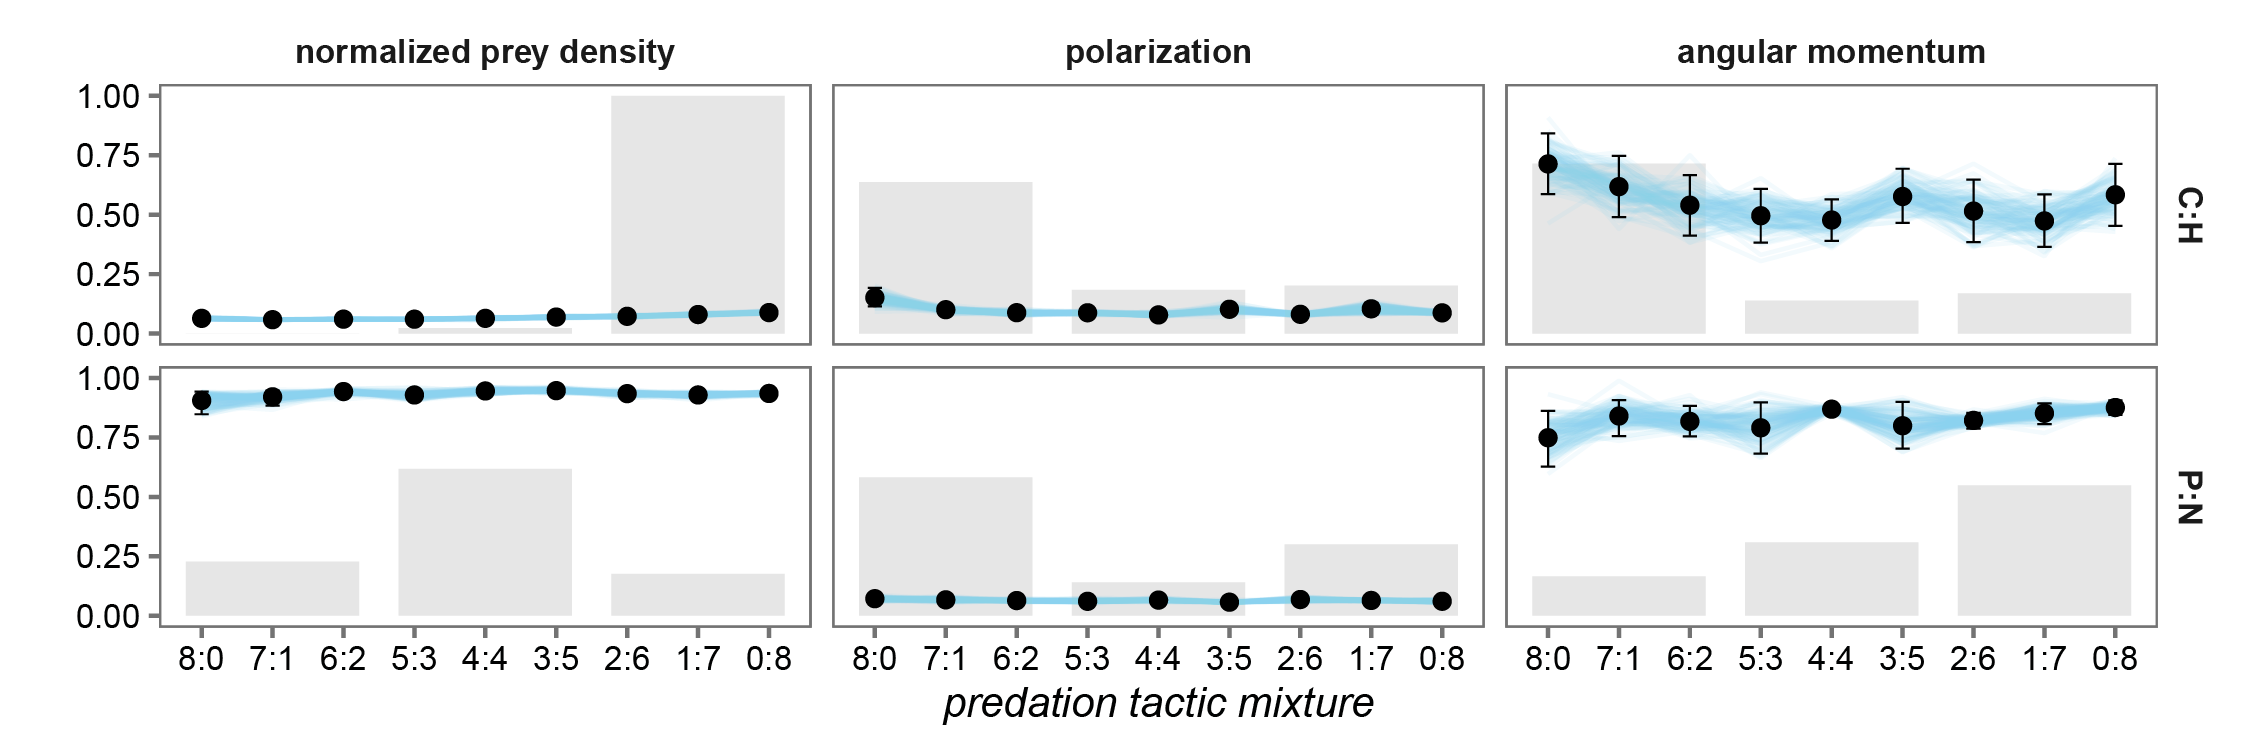
\includegraphics[width=\figurewidth]{scirep/dpm_conforming}
	\infigurecaption{P -- attack prey individuals located at the periphery of prey groups, N -- attack the nearest prey individual, C -- attack the most central prey individual in a prey group, and H -- high density area attacks. The predation pressure mixture ratio \emph{a}:\emph{b} denotes the number of predators using a specific predation tactic, \eg in the case of C:H, 0:8 (top row, right side of the plot) all predators (eight) use high density area attacks. Points and whiskers represent the estimated posterior means and 95\% posterior confidence intervals. Individual draws from the posterior distributions are connected with lines to visualize posterior uncertainty and aid in the interpretation of how the means vary across the predation pressure mixtures. To summarize the results, the predation mixtures were grouped into groups of three: predation pressure predominantly from centre (C:H) or periphery (P:N) attacking predators (8:0, 1:7, 2:6), balanced pressure (5:3, 4:4, 3:5), and predation pressure predominantly from high density area (C:H) or nearest prey individual (P:N) attacking predators (6:2, 7:1, 0:8). The shaded bars show, for each group, the probability that that group has the highest mean. These probabilities were estimated with draws from the posterior distributions in which each group member had an equal probability of being selected. That is, each predation mixture was weighted equally.}
	\caption{Normalized prey density, polarization, and angular momentum for conforming predation pressure mixtures.}	\label{figure:conforming}
\end{figure}

According to previous studies \cite{biswas2014causes,kunz2006prey,olson2013predator,olson2016evolution} predation pressure from predators that attack the most central prey individual in a prey group (C) or use high density area attacks (H) should promote the evolution of the tendency to disperse in prey individuals. On the other hand, predation pressure from predators that attack prey individuals located at the periphery of the prey groups (P) or the nearest prey individual (N) should lead to the evolution of the tendency to group. As from the point of view of the expected outcome in both cases the two predation tactics agree, regardless of the number of predators using a specific tactic (dispersion for combination C:H, grouping for P:N), we call such predation pressures conforming. Our results (\figurename~\ref{figure:conforming}) support previous studies. With conforming pressures towards dispersing by centre and density attacking predators the mean normalized prey density consistently stayed below \num{0.125}, regardless of the number of predators using a specific tactic. On the other hand, with conforming pressures towards grouping by periphery and nearest prey individual attacking predators the mean normalized prey density remained above \num{0.75}, regardless of the number of predators using a specific tactic.

Couzin\etal \cite{couzin2002collective} introduced the measures of polarization and angular momentum. They express the degree of consensus in a common heading of the group (polarization), and the degree of rotation of the group about the group's centre (angular momentum). By means of these two measures Couzin\etal \cite{couzin2002collective} defined four collective dynamical behaviours: swarm (low polarization and low angular momentum), torus or milling (low polarization and high angular momentum), dynamic parallel group (high polarization and low angular momentum), and highly parallel group (very high polarization and low angular momentum) \cite{couzin2002collective}. 

Conforming predation pressures (combinations C:H and P:N in \figurename~\ref{figure:conforming}) resulted in behaviours with medium to high angular momentum and low polarization. While polarization was low for all pressure mixtures, its mean was highest when predation pressure came predominantly from centre or periphery attacking predators. Predation pressures for which the response was grouping led to consistently high angular momentum with low variability. Here attacks directed predominantly on the nearest prey individual gave rise to the highest mean angular momentum. The high angular momentum combined with the consistently low polarization suggests the evolution of milling behaviours. Pressure towards dispersing, on the other hand, resulted in substantially lower angular momentum with a higher variability. Here, domination by centre attacking predators induced the highest mean angular momentum. As polarization was low the medium to high angular momentum with high variability suggests the evolution of either swarming or milling behaviours. Note here that even in cases where polarization was the highest it was not high enough to suggest the observed behaviour could be classified as polarized.

\begin{figure}
	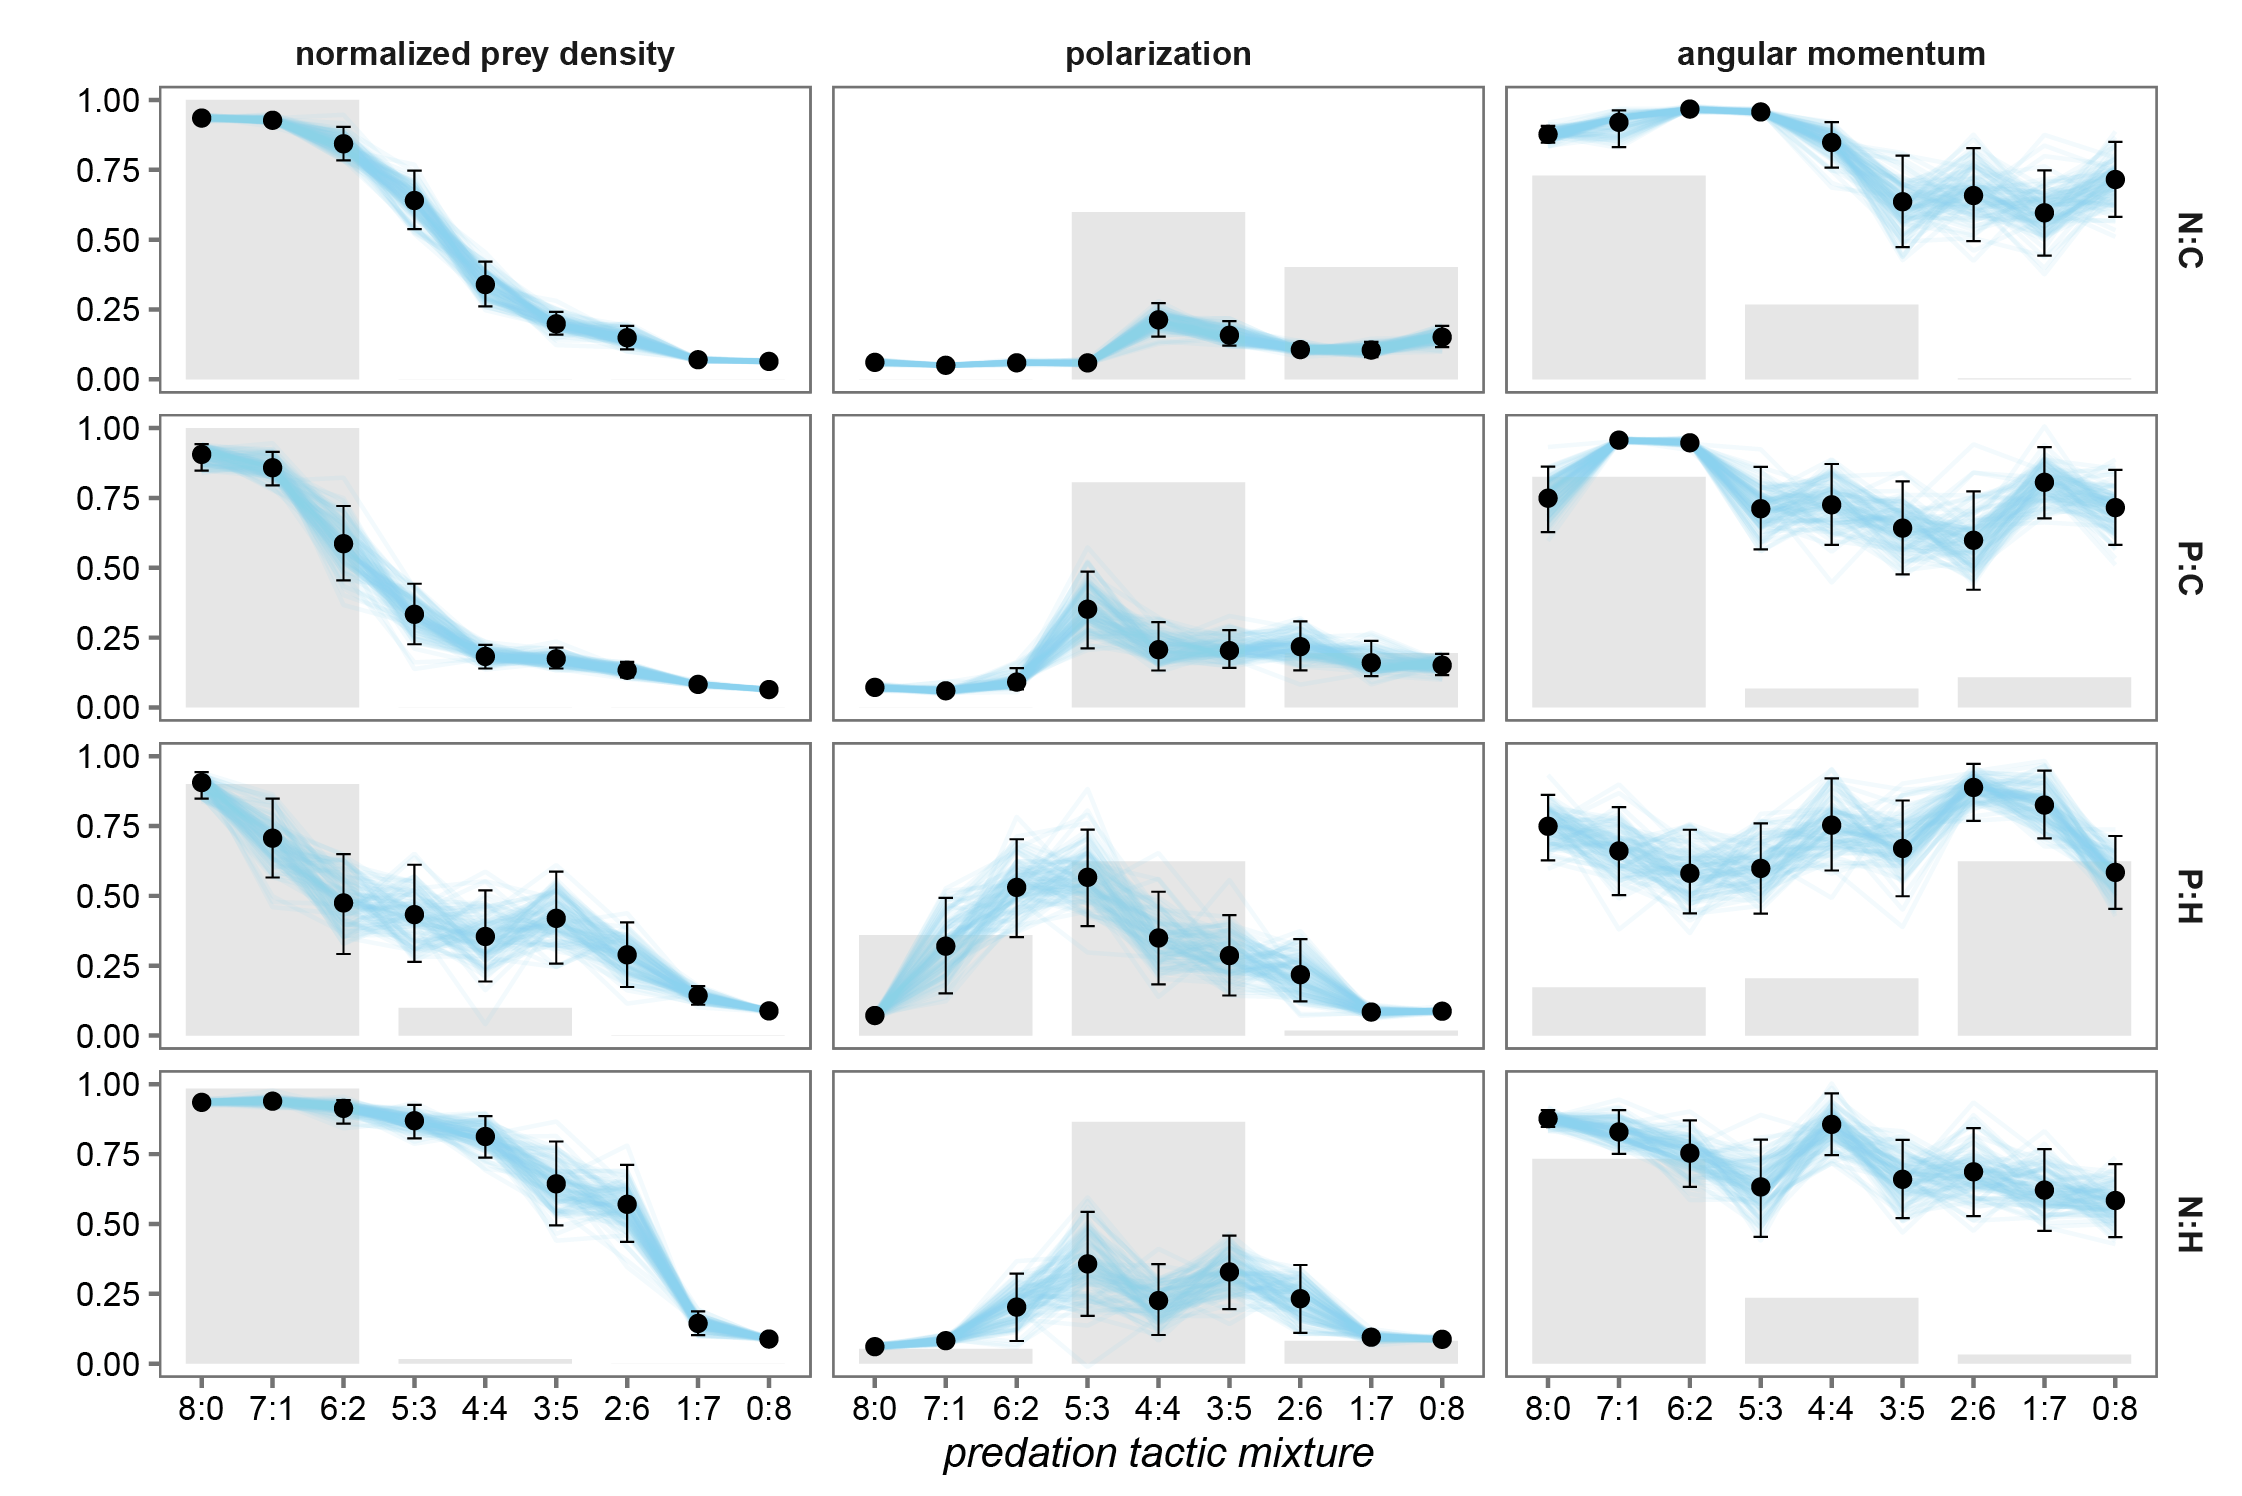
\includegraphics[width=\figurewidth]{scirep/dpm_antagonistic}
	\infigurecaption{P -- attack prey individuals located at the periphery of prey groups, N -- attack the nearest prey individual, C -- attack the most central prey individual in a prey group, and H -- high density area attacks. The predation pressure mixture ratio \emph{a}:\emph{b} denotes the proportion of predators using a specific predation tactic, \eg in the case of N:C, 0:8 (top row, right side of the plot) all predators (eight) attack the most central prey individual in a prey group. Points and whiskers represent the estimated posterior means and 95\% posterior confidence intervals. Individual draws from the posterior distributions are connected with lines to visualize posterior uncertainty and aid in the interpretation of how the means vary across the predation pressure mixtures. To summarize the results, the predation mixtures were grouped into groups of three: low degree of antagonism in predation pressures with predominant pressure from predators that force prey into grouping (8:0, 1:7, 2:6), high degree of antagonism in predation pressures (5:3, 4:4, 3:5), and low degree of antagonism in predation pressures with predominant pressure from predators that force prey into dispersion (6:2, 7:1, 0:8). The shaded bars show, for each group, the probability that that group has the highest mean. These probabilities were estimated with draws from the posterior distributions in which each group member had an equal probability of being selected. That is, each predation mixture was weighted equally.}
	\caption{Normalized prey density, polarization, and angular momentum for antagonistic predation pressure mixtures.}
	\label{figure:antagonistic}
\end{figure}

In the case of antagonistic predation pressures (combinations N:C, N:H, P:C and P:H, see \figurename~\ref{figure:antagonistic}) the highest mean normalized prey density emerged when predation pressure came predominantly from the nearest or the most peripheral prey individual attacking predators (predators that in a conforming setting pressure prey into grouping; mixtures 8:0, 7:1, 6:2). On the other hand, domination by predators for which the expected outcome is dispersing (mixtures 2:6, 1:7, 0:8) led to the lowest mean normalized prey density. Domination by either pressure to group or pressure to disperse can be interpreted as a low degree of antagonism in predation pressures. A high degree of antagonism, where neither the pressure to disperse nor the pressure to group dominates (mixtures 5:3, 4:4, 3:5), led to the evolution of low to high mean normalized prey density. The lowest in the case of periphery and centre attacking predators (P:C) and highest in the case of nearest prey individual and high density area directed attacks (P:H).

Evolution under antagonistic predation pressures resulted in medium to high angular momentum and low to medium polarization. Compared to the case of conforming predation pressures, there was a considerably higher variability in the values of angular momentum and polarization, suggesting a wider range of evolved behaviours. In all but the P:H case, predation pressure predominantly from predators that result in prey individuals that favour grouping gave rise to the highest angular momentum. In the P:H case, on the other hand, it was highest when the pressure to disperse dominated. Note that angular momentum was never the highest when antagonism in predation pressures was high (predation pressure mixtures 5:3, 4:4, 3:5). High antagonism, however, always generated the highest mean polarization.

Observing all three parameters in unison (see Supplementary information, \figurename~\ref{figure:antagonistic:SM}) suggests that increasing the pressure towards dispersing from centre or high density area attacking predators leads to a general decrease in normalized prey density, angular momentum and polarization (top and right portion of the figure). An increase in pressure towards grouping from predators that attack the nearest or the most peripheral prey individual, on the other hand, causes an increase in density and a favouring of higher momentum with low polarization (bottom and left portion of the figure). Higher values of polarization with low momentum and medium density emerge when the mixture in pressures towards and against grouping (towards dispersing) is somewhat balanced. This suggests a possible emergence of polarized behaviour. 

\begin{figure}
	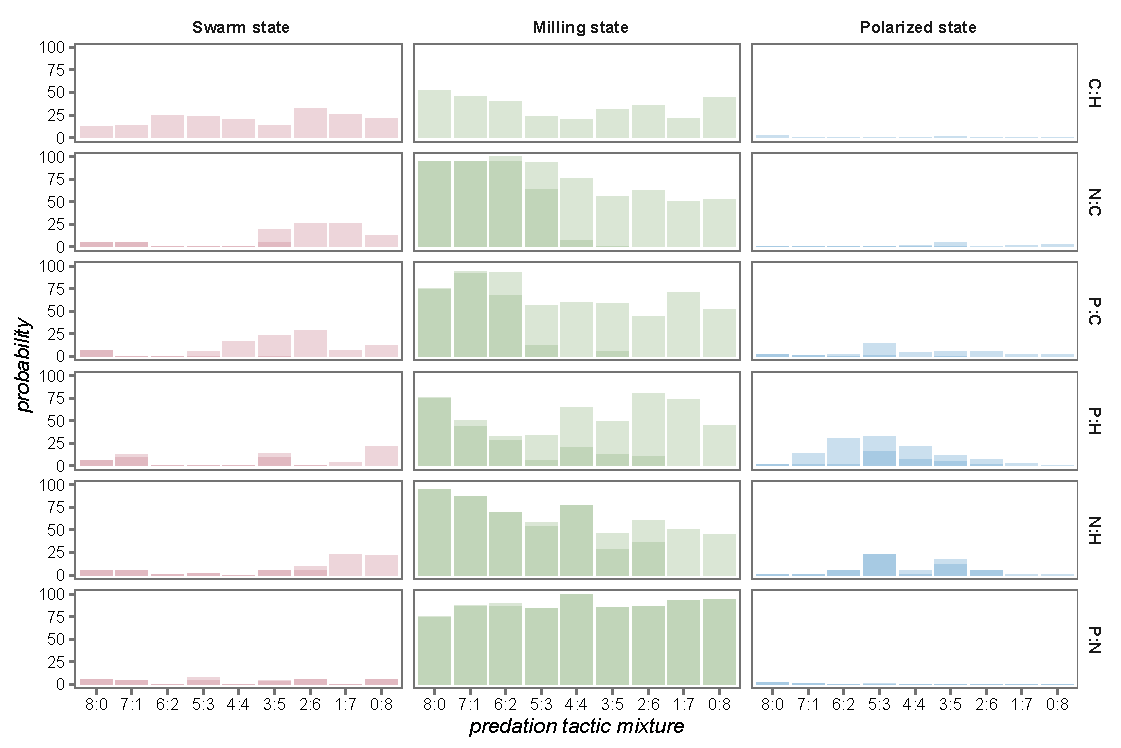
\includegraphics[width=\linewidth]{scirep/class_t__35_1800_final}
	\infigurecaption{P -- attack prey individuals located at the periphery of prey groups, N -- attack the nearest prey individual, C -- attack the most central prey individual in a prey group, and H -- high density area attacks. The shading denotes cases with low (light shading) and high normalized prey density (dark shading). The predation pressure mixture ratio \emph{a}:\emph{b} denotes the proportion of predators using a specific predation tactic, \eg in the case of C:H, 8:0 (top row, left side of the plot) all predators (eight) attack the most central prey individual in a prey group.}
	\caption{The probability of observing a specific collective state at the end of the simulation run for all predation pressure mixtures.}
	\label{figure:classification}
\end{figure}

Note that polarization and angular momentum reported in \figurename s~\ref{figure:conforming}, \ref{figure:antagonistic} and \ref{figure:antagonistic:SM}, although indicative of the resulting behaviour, cannot be used for such a classification directly, because they were computed as weighted sums of polarization and angular momentum of individual groups and averaged over a number of frames (see Methods). Therefore, to further analyse the influence of predation pressures on the evolution of prey behaviour, we categorized the behaviour of individual groups with respect to their polarization and angular momentum in the last frame of of every simulation run. Here we followed Tunstrøm\etal \cite{tunstrom2013collective}, who used polarization and angular momentum and a simple threshold to categorize the behaviour of groups of golden shiners, \emph{Notemigonus crysoleucas}, into one of three collective states; swarm, milling, and polarized state. Based on that we computed the probability of observing a particular collective state (see Methods). This analysis provides further insight into what kind of behaviour evolves under a particular predation pressure mixture ratio. \figurename~\ref{figure:classification} confirms what was suggested by data presented in \figurename s~\ref{figure:conforming}, \ref{figure:antagonistic} and \ref{figure:antagonistic:SM}: the probability of observing the swarm state is present mainly in cases when prey individuals evolved while under predation pressure from centre or high density area attacking predators. The probability of observing a swarm state is the highest when prey individuals evolved under conforming pressures towards dispersing by centre and density attacking predators. Overall, the probability of observing a milling state dominates, and is high in most cases, except when: a) prey individuals evolved under conforming pressures towards dispersing by centre and density attacking predators, and b) prey individuals evolved under certain antagonistic pressures. On the other hand, evolution under antagonistic pressures produced the highest probability of observing a polarized state. This suggests that a mixture of antagonistic pressures that simultaneously steer prey towards grouping and dispersing might be required for prey individuals to evolve parallel movement.

Visual inspections of the evolved behaviours confirmed that the domination of predation pressures towards dispersing led prey to evolve behaviours where they in general tend to disperse. This tendency to disperse at times leads to the wall-following of the living area border and thus while keeping a low density causes a relatively high angular momentum (see Supplementary information, \videoname~\ref{video:V1}). As this is classified as milling, the probability of observing the milling state dominates in \figurename~\ref{figure:classification}. The solution being classified as milling is probably irrelevant for biological organisms as it is determined by the artificial ecology used for this computational study (\ie crossing the living area border would sooner or later be lethal for the prey individual). Nevertheless, in an experiment with zebrafish, \emph{Danio rerio}, the distribution of the positions detected in the tank showed that the fish avoid the centre of the tank and the higher probability of presence is along the walls \cite{collignon2016stochastic}, which might be indicative of a similar form of wall-following. On other occasions with low density the evolved behaviour resembled collective motion typically identified as swarming, associated with low angular momentum, and low polarization (see Supplementary information, \videoname~\ref{video:V2}). Predation pressure predominantly from predators that push prey into grouping led prey individuals to evolve behaviours that usually resulted in high density, high angular momentum and low polarization, values typically associated with milling (see Supplementary information, \videoname~\ref{video:V3}). On few occasions the evolved behaviour resulted in high density, low angular momentum and low polarization, indicative of high density swarming (see Supplementary information, \videoname~\ref{video:V4}). As suggested by data presented in \figurename s~\ref{figure:antagonistic} and \ref{figure:classification} behaviours with higher values of polarization emerged mostly when there was a high degree of antagonism in predation pressures (\ie when there was a balanced mixture of pressure towards and against grouping). Here prey individuals often evolved behaviours that resulted in parameter values typical for dynamic and highly parallel motion; medium to high normalized density, low to medium angular momentum and medium to high polarization (see Supplementary information, \videoname s~\ref{video:V5}--\ref{video:V7}).

%-----
\section{Discussion}

Previous research that used evolutionary computational models to study the evolution of collective behaviour \cite{biswas2014causes,kunz2006prey,morrell2015consequences,olson2013predator,olson2016evolution} suggests that prey grouping might have evolved as a defensive mechanism against predation. Most of the existing studies were principally interested in whether prey evolve a) grouping behaviour (defined as an increase in prey density) or b) dispersing behaviour (defined as a decrease in prey density). Our study corroborates previous findings in that prey density is high when prey individuals evolve while under predation pressure from predators for which grouping might be a natural response (attack peripheral prey individuals, or attack the nearest prey individual), and low when prey individuals evolve while under predation pressure from predators for which dispersing might be a natural response (attack the most central prey individual, or attack high density areas).

Groups of animals in nature, however, move in many different fashions (clumping, swarming, milling, schooling, etc.) \cite{krause2002living,suzuki1973movement} and different predation pressures are countered by different responses. As these responses are experience dependant \cite{elmasri2012response,hellstrom2016balancing}, we can hypothesise that if collective behaviour evolved as an anti-predator response it might as well have been shaped by the predation pressures the prey faced. In this study we therefore expanded on previous research by focusing on how predation from various types of predators might influence the evolution of collective behaviour in prey individuals. More specifically we investigated the influence of antagonism between predation pressures towards and against grouping (towards dispersing) on the type of evolved collective behaviour (evaluated via prey density, polarization and angular momentum \cite{couzin2002collective}). Our results suggest that when prey individuals evolve while under conforming predation pressures (either towards grouping or towards dispersing) the resulting behaviour has low polarization and medium to high angular momentum. When prey individuals evolve while subject to antagonistic predation pressures (towards grouping and towards dispersing, simultaneously) density and angular momentum increase with the number of predators forcing prey into grouping and decrease with the number of predators that force prey individuals into dispersing. Polarization, on the other hand, is highest when antagonism in predation pressures is high.

Our results therefore suggest that antagonism might have played an important role in the evolution of collective behaviour; that antagonism from predation pressures, environmental or internal factors could have been responsible for the evolution of a multitude of different behaviours. They could also indicate that in nature the evolution of highly polarized movement might be a result of the co-evolution of prey evasion and composite predator attack tactics \cite{demsar2015simulating}. Another possibility is that not only variation in swimming performance \cite{oufiero2016evolution}, but also the amount of variation in group behaviours might be linked to environmental factors. This supports the hypothesis that ecological constraints may shape the process used to regulate activity in many biological species \cite{gordon2014ecology}. Indeed, evolution of group responses to predation in nature is not universal, and different species might evolve very different responses to predation. This is not restricted to fish schools, as it is evident also in avian group behaviour, where the magnitude in variation of behaviours has always been a major puzzle. Why do so few bird species that fly together display organized behaviour, and why do even closely related species display major differences in flocking behaviour \cite{lebarbajec2009organized}. For example, pigeons are more closely related to swifts than they are to starlings \cite{jarvis2014wholegenome}, but they flock much more like starlings. Similarly, geese are more closely related to chickens than they are to cormorants \cite{jarvis2014wholegenome}, but they fly like cormorants.\footnote{Heppner FH, \emph{personal communication}, February, 2016} In view of our results one possible explanation for these observations might be that organized flight has evolved independently, and several times, and the differences in behaviour might have emerged because, although closely related, individual species were subject to different pressures.

In marine ecology Rieucau\etal's recent studies suggest that collective anti-predator responses in herring increase with the density of the school \cite{rieucau2014School}, and the number of sensory cues \cite{rieucau2014experimental,rieucau2015herring}. Our results suggest that the increase might be accentuated by the conflict in sensory cues. This corroborates recent results by Lemasson\etal \cite{lemasson2016sensory}, who suggest that the benefits of coordinated motion are context dependent, \ie they can potentially reduce the time prey individuals spend in dangerous areas and help them to avoid becoming isolated, yet such movement patterns can also alleviate predator confusion during a directed attack. It is important to note that exposure to predators affects prey both directly and indirectly and that plasticity in response to risk might relate to an individual's willingness to take risks \cite{abbeylee2016behavioral}. As our model is heterogeneous in the behaviour of prey individuals, our findings seem to suggest that this individuality in susceptibility to predation risk, might inevitably also lead to changes in the behaviour of the group.

In summary, while the dilution of risk might be sufficient for prey individuals to evolve grouping \cite{biswas2014causes}, and predator confusion might lead prey individuals to evolve swarming \cite{kunz2006prey,olson2013predator,olson2016evolution}, our results suggest that exposure to antagonistic predation pressures might be a necessary requirement for prey individuals to evolve parallel movement. This could indicate that the direction of evolution (grouping or dispersing) is not A versus B, but a labile result -- whether grouping or dispersing evolves depends on a) the nature of the group, and b) the pressures that the group finds itself facing.

%-----
\section{Methods}

Our individual based model consists of two types of artificial animals -- predators and prey. They coexist in a two dimensional environment confined by a circular living area, with their positions and headings at time instant $t$ given by $\vec{r}^{(i)}_t$, $\phi^{(i)}_t$. Following previous research \cite{dellorco2014simulation,demsar2014simulated,lebarbajec2005simulating,lucic2002transportation,tron2004mathematical}, the behaviour of every artificial animal in our model is governed by fuzzy logic \cite{zadeh1965fuzzy} via a fuzzy-rule-based system \cite{mamdani1974application}. A fuzzy-rule-based system enables the use of linguistic if-then rules to describe the behaviour of the artificial animals. It is specified via a fuzzy knowledge base, which consists of a fuzzy data base and a fuzzy rule base. The data base lists all input and output variables, as well as the linguistic terms (\eg near, far, etc.) that can appear in if-then rules. In addition it includes information necessary for fuzzy reasoning, \ie the method for transforming crisp data into fuzzy sets (fuzzification), the interpretation of logical connectives necessary for fuzzy reasoning, and the method for converting the fuzzy result into a real action (defuzzification). The fuzzy rule base on the other hand comprises the list of if-then rules that are assumed to be joined by the connective ``also,'' so multiple rules can fire simultaneously. When used in combination with artificial evolution a fuzzy-rule-based system is called a genetic fuzzy system \cite{cordon2004ten,fernandez2015revisiting,herrera2008genetic}. 

The fuzzy knowledge base of the predators was set following previous research \cite{demsar2014simulated} (see Supplementary information for details). In the case of prey individuals we, for reasons of simplicity, locked the fuzzy data base and evolved only the fuzzy rule base (see Supplementary information for details), but given that fuzzy-rule-based systems are deemed universal approximators \cite{castro1995fuzzy} this still provides the opportunity to potentially discover a wide repertoire of behaviours. 

At every update step the fuzzy-rule-based systems (\ie the pre-set fuzzy knowledge base in the case of predators, and the evolving fuzzy knowledge bases in the case of prey individuals) were used to compute the new heading (see \figurename~\ref{figure:FS}) and position of every artificial animal as:
%
\begin{figure}
  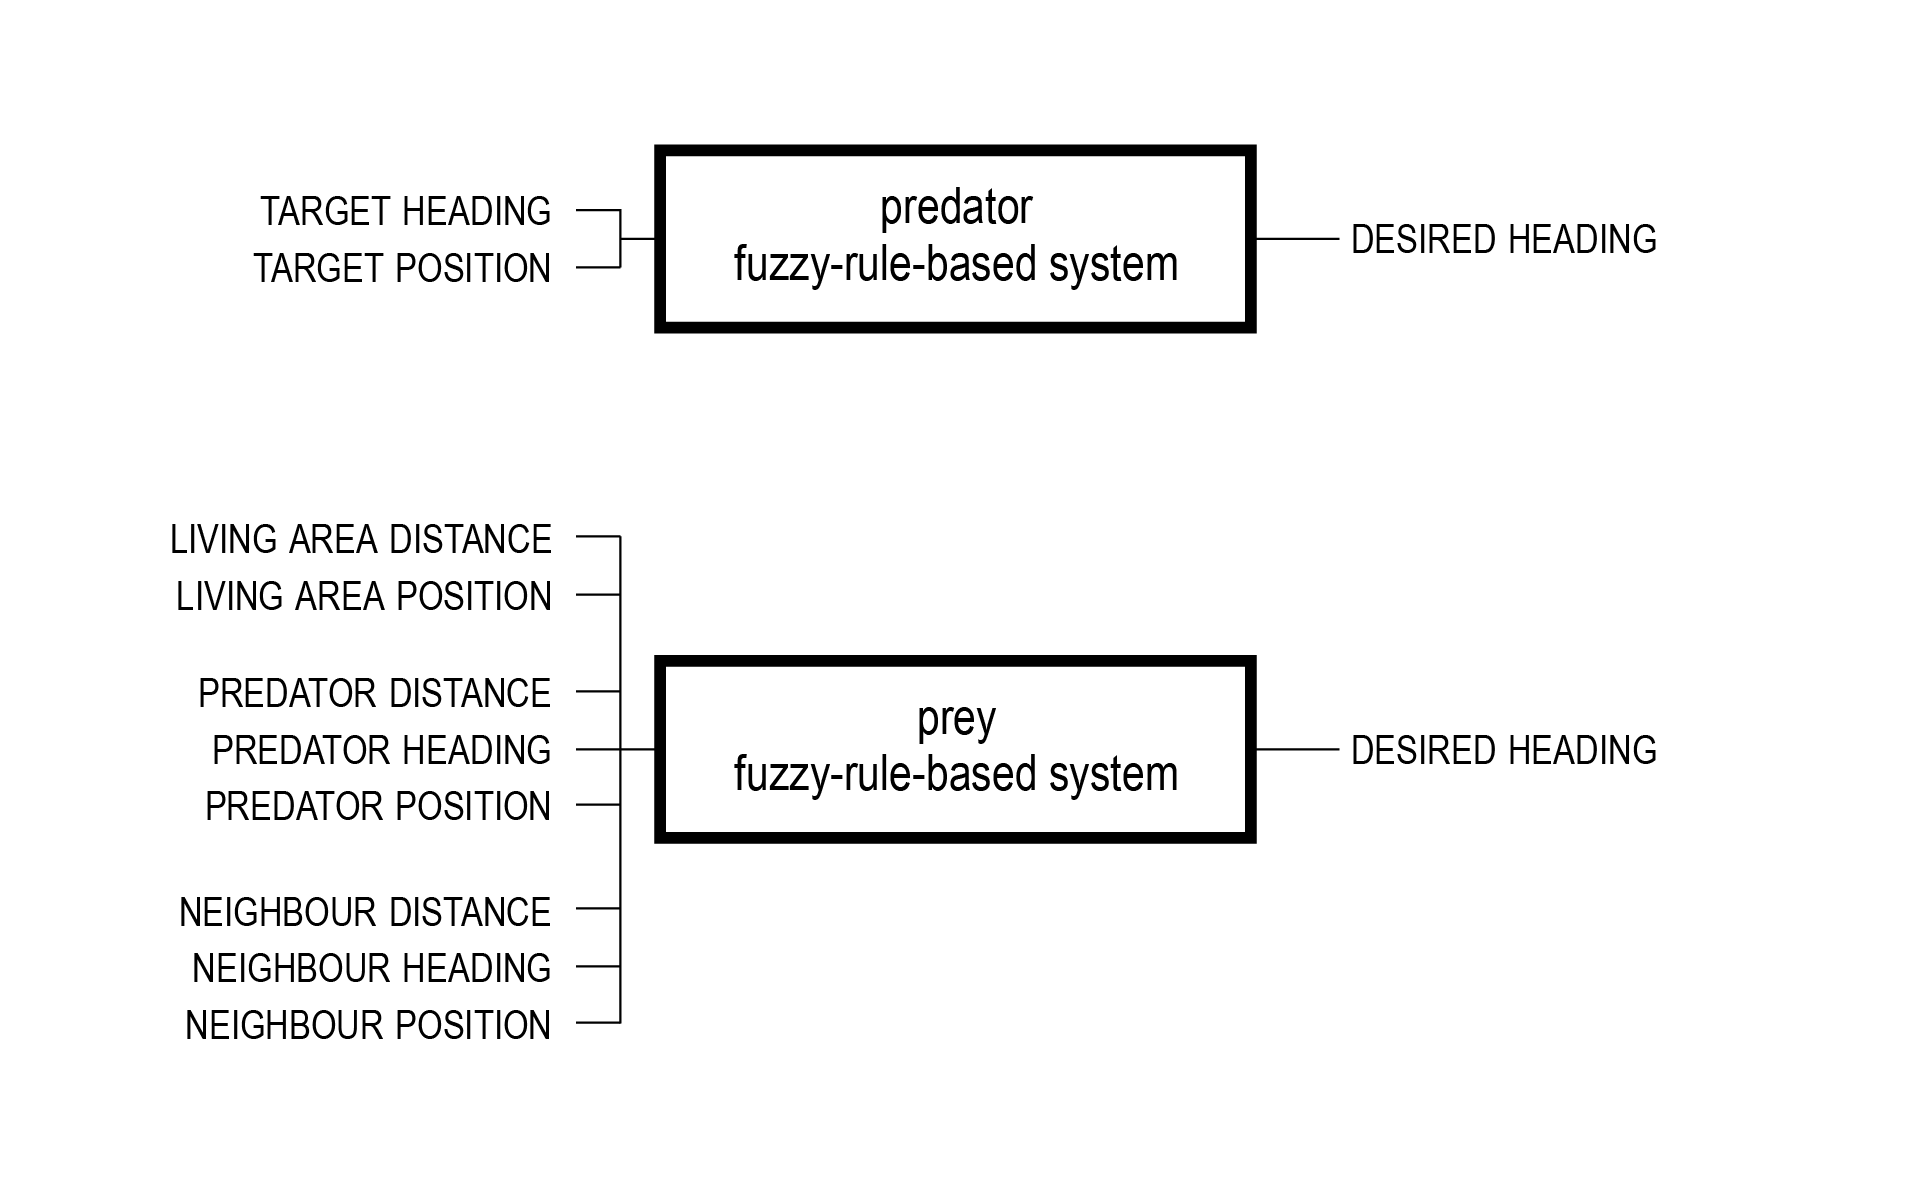
\includegraphics[width=.75\linewidth]{scirep/FS}
  \caption{A schematic showing the predator and prey fuzzy-rule-based system's input and output variables.}
  \label{figure:FS}
\end{figure}
%
\begin{equation}
%\omega^{(i)}_{t+\tau}= \min(\phi^{(i)}_t - \phi^{(i)}_\textnormal{FS},\ \omega^{(i)}_\textnormal{max}),
\omega^{(i)}_{t+\tau}= \min(\phi^{(i)}_\textnormal{FS},\ \omega^{(i)}_\textnormal{max}),
\end{equation}
%
\begin{equation}
\phi^{(i)}_{t+\tau}=\phi^{(i)}_t + \tau\omega^{(i)}_{t+\tau},
\end{equation}
%
\begin{equation}
\vec{v}^{(i)}_t=v^{(i)}\begin{bmatrix}\cos\phi^{(i)}_t \\ \sin\phi^{(i)}_t\end{bmatrix},
\end{equation}
%
\begin{equation}
\vec{r}^{(i)}_{t+\tau}= \vec{r}^{(i)}_t + \tau\vec{v}^{(i)}_{t+\tau},
\end{equation}
%
where $\phi^{(i)}_\textnormal{FS}$ is the desired heading in the local coordinate frame of individual $i$ returned by the corresponding fuzzy-rule-based system, $\omega^{(i)}_\textnormal{max}$ is its manoeuvrability and $v^{(i)}$ is the animal's speed. See Supplementary information, \tablename~\ref{table:parameters:SM}
for a full list of parameters. The following sections provide more details about the evolutionary process and analysis of the evolved behaviour. For more details about the implementation of the predator and prey artificial animal see Supplementary information.

%-----
\subsection{Evolutionary process}

Most of the previous studies concerning the evolution of collective behaviour \cite{kunz2006prey,olson2013predator,olson2016evolution,wood2007evolving} used a genetic algorithm, with clearly defined generational boundaries. This is the most frequently used application of genetic algorithms, where in every generation the whole population of potential solutions to the problem is evaluated via simulation in order to evaluate the fitness (assess the quality) of every individual solution. The fitness is then used for selection, followed by reproduction and mutation so that the whole population of possible solutions is created anew and is defined as a new generation. Additionally, with the only exception of Wood \& Ackland \cite{wood2007evolving} in most of the previous studies \cite{kunz2006prey,olson2013predator,olson2016evolution} all of the prey individuals behaved in exactly the same way -- the prey groups were homogeneous.

Some recent studies suggest that heterogeneous groups might evolve a different behaviour in an algorithm mimicking artificial evolution \cite{olson2015exploring}. Others suggest that heterogeneous groups might be necessary to achieve a more ``natural'' behaviour \cite{demsar2013family}, and that differences among individuals might be essential for group coordination \cite{marras2012information,marras2013schooling}. For this reason in our approach, similar to Biswas\etal \cite{biswas2014causes}, selection, followed by reproduction and mutation are part of the simulation so that there is no clear generational boundary. When a prey individual (a potential solution to the problem) in our system dies, two of the remaining prey individuals are selected based on their current fitness, and via reproduction and mutation a new prey individual is created (a new potential solution to the problem). Since every prey individual is governed by its own fuzzy-rule-based system, this essentially makes the prey group heterogeneous.

The fitness of a prey individual was evaluated via its energy level $\epsilon^{(i)}_t$, which encodes the individual's capability to stay in the designated living area, avoid collisions with other prey individuals, and successfully avoid predation. When a new prey individual was created, it was assigned an initial level of energy, $\epsilon_0$, and with every update step the energy level was increased by $\epsilon_\textnormal{l}$. As in the case of Kunz\etal \cite{kunz2006prey} inter-prey collisions were penalized to promote collision avoidance, \ie in the event of a collision the energy level of the involved prey individuals was decreased by $\epsilon_\textnormal{c}$. Similarly, to promote staying inside the living area, wandering outside of it (\ie $\|\vec{r}^{(i)}_t\| \geq r_\textnormal{LA}$) was penalized by $\epsilon_\textnormal{w}$. A prey individual died if its energy level depleted to 0 or was marked as captured by a predator (see Supplementary information). Since a new prey individual was created (\ie it appeared at a random location heading in a random direction) whenever one died, the number of prey individuals was constant throughout the entire evolution.

Individual predators appeared at random time instants at random locations outside of the living area. Their initial heading was towards the centre of the living area, so as to promote the speed of convergence of the evolutionary algorithm \cite{olson2016evolution}. High density area attacking predators hunted until their hunt duration elapsed. Single-target (neatest, centre, and periphery) attacking predators hunted until they caught the currently targeted prey individual, or until their hunt duration elapsed. Once a predator finished its hunt, it was removed, and re-appeared after a random time interval. The initial delay before a predator first appeared, and the time interval before it re-appeared after a hunt were uniformly distributed on the predator re-appearance time interval, $t_\textnormal{r}$. At maximum eight predators were simultaneously present at one time instant. 

In order to investigate the type of evolved behaviour when varying exposure to conforming and antagonistic predation pressures we ran individual evolutions while varying the number of predators using a specific predation tactic. In total we ran 54 experiments with different conditions (mixtures of different predation pressure combinations). Each evolutionary run lasted ten million update steps and was repeated 20 times.

%-----
\subsection{Analysis of the evolved behaviour}

\begin{figure}
  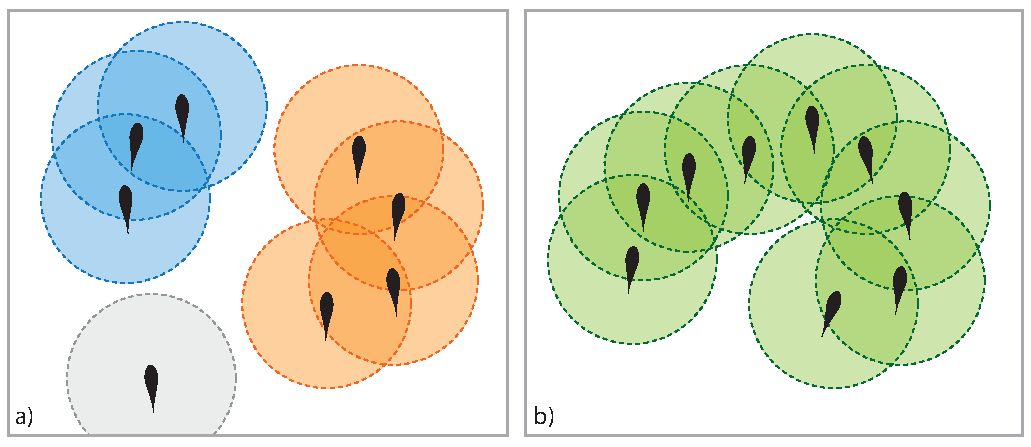
\includegraphics[width=\figurewidth]{scirep/preyGroups}
  \infigurecaption{a) one straggler and two proper groups; the straggler does not see any prey individual from either of the two groups, and no member from one group is able to see neither the straggler nor any prey individual from the other group; potential influence (direct or indirect) is limited to members of the same group only; b) one proper group where all members can potentially (directly or indirectly) influence each other's behaviour.}
  \caption{Prey individuals split into groups based on direct and indirect influence.}
  \label{figure:groups}
\end{figure}

To classify the evolved behaviour we ran five separate simulation runs where on each occasion the artificial world comprised only the prey individuals from the last update step of the corresponding evolutionary run. This was done to preclude the possibility of the behaviour being classified as collective, when in reality all prey are individually trying to escape the predator in a common direction, hence we analysed the evolved behaviour with no predator present. Each simulation run lasted 1800 update steps and on each occasion the type of behaviour was analysed after it reached a dynamically stable state (\ie after 900 update steps). For the analysis we turned to the observation of density \cite{olson2016evolution}, polarization, and angular momentum \cite{couzin2002collective}, properties that allow for the categorization of the type of collective behaviour \cite{couzin2002collective,olson2016evolution,tunstrom2013collective,vicsek2012collective,wood2007evolving}. Density, \eq~\eqref{equation:density}, can be used to assess the degree of grouping, or clumping. Polarization, \eq~\eqref{equation:polarization}, express the degree of consensus in a common heading. Angular momentum, \eq~\eqref{equation:momentum}, the degree of rotation of the group about the group's centre. Together they can be used to assess the type of collective behaviour (\ie swarm, torus, dynamic parallel group, or highly parallel group) \cite{couzin2002collective}. The quantities were recorded over the remaining 900 update steps of a simulation, and their individual averages were used as an indication of the evolved behaviour. 

Normalized prey density
%
\begin{equation}
    \rho_t = \frac{1}{\left|\set{I}\right|^2 - \left|\set{I}\right|} \sum_{i \in \set{I}}{\left|\set{N}^{(i)}_t\right|},\quad \set{N}^{(i)}_t=\{j \in \set{I}|\ j \neq i, \|\vec{r}^{(j)}_t - \vec{r}^{(i)}_t\| \leq r^{(i)}_\textnormal{v}\}
	\label{equation:density}
\end{equation}
%
where $\set{N}^{(i)}_t$ is the neighbourhood of prey individual $i$, was recorded on a global level. However, in view of recent research \cite{viscido2015using}, which emphasizes the importance of calculating the observed quantities on a group-by-group basis, for polarization and angular momentum the prey individuals were first split into groups based on direct and indirect influence (see \figurename~\ref{figure:groups}) \cite{lebarbajec2007boids}, where
%
\begin{equation}
\text{1. }\set{G}^{(i)}_t \subseteq \set{I},\quad \text{2. }i \in \set{G}^{(i)}_t,\quad \text{3. if } j \in \set{G}^{(i)}_t \text{ then, } \set{N}^{(j)}_t \subset \set{G}^{(i)}_t, 
\end{equation}
%
is a recursive definition of a group of prey individuals. Prey individuals pertaining to groups of size one, $\sset{S}=\{i \in \set{I}|\ \left|\set{G}^{(i)}_t\right| = 1\}$, are termed stragglers \cite{lebarbajec2007boids} and proper groups can be defined as
%
\begin{equation}
\sset{G}=\{i_1,\ldots,i_n\}:\ \bigcup_{i \in \sset{G} \cup \sset{S}}\set{G}^{(i)}_t = \set{I},\ \forall i,j \in \sset{G}:\ \set{G}^{(i)}_t \cap \set{G}^{(j)}_t = \emptyset.
\end{equation}

Polarization and angular momentum were computed based on proper groups only and in order to diminish the possible bias induced by many small groups the two quantities at time instant $t$ were computed as weighted averages, where group size was used as the weighting function. Hence polarization was computed as
%
\begin{equation}
p_t = \sum_{g \in \sset{G}}{\frac{\left| \set{G}^{(g)}_t\right|p^{(g)}_t}{\left|\cup_{g \in \sset{G}}\set{G^{(g)}_t}\right|}},\quad p^{(g)}_t = \frac{1}{\left|\set{G^{(g)}_t}\right|}{\left\| \sum_{i \in \set{G}^{(g)}_t}{\uvec{v}^{(i)}_t} \right\|},
\label{equation:polarization}
\end{equation}
%
and angular momentum as
%
\begin{equation}
m_t = \sum_{g \in \sset{G}}{\frac{\left| \set{G}^{(g)}_t\right|m^{(g)}_t}{\left|\cup_{g \in \sset{G}}\set{G^{(g)}_t}\right|}},\quad  m^{(g)}_t = \frac{1}{\left|\set{G}^{(g)}_t\right|}{\left\| \sum_{i \in \set{G}^{(g)}_t}{\uvec{r}^{(\set{G},i)}_t \times \uvec{v}^{(i)}_t} \right\|},
\label{equation:momentum}
\end{equation}
%
where $p^{(g)}_t$ and $m^{(g)}_t$ are the polarization and angular momentum of group $g$, respectively and 
%
\begin{equation}
\vec{r}^{(\set{G},i)}_t=\vec{r}^{(i)}_t - \frac{1}{\left|\set{G}^{(i)}_t\right|}\sum_{j \in \set{G}^{(i)}_t}{\vec{r}^{(j)}_t}
\end{equation}
%
is the relative position of prey individual $i$ with respect to the centroid of its group.

%-----
\subsection{Statistical analysis}

The main goal of our experiments (evolution + simulation) was to investigate how the mean of three metrics of interest (normalized prey density, polarization and angular momentum) varies across six different pairs of the four predation tactics (C:H, N:C, P:C, P:H, N:H, P:N) and nine different predation mixtures (8:0, 7:1, ..., 0:8). 

Each combination of the three dimensions above is considered a separate experiment. The experiments are not deterministic -- both the evolution and simulation are stochastic in nature and therefore a source of (random) measurement error. To estimate and account for this, each experiment consisted of $n=20$ different evolutionary runs (iterations), each followed by $m=5$ simulation runs (repetitions). The metrics also vary across individual frames, however, low variability and a relatively high number of frames (900) leads to a negligible standard error, therefore, instead of modelling individual frames, the average across all frames was used.

For each experiment separately, we used the following Bayesian hierarchical model to estimate the mean:
%
\begin{equation}
\begin{split}
y_{ij} &\sim \mathcal{N}(\mu_i, \sigma_i)\\
\mu_{i} &\sim \mathcal{N}(\mu_0, \sigma_0)\\
\mu_0 &\propto 1 \\
\log \sigma_\cdot &\propto 1,
\end{split}
\end{equation}
%
where $y_{ij}$ is the metric measurement for the $j$-th repetition of the $i$-th iteration. That is, we model each iteration with its own distribution with potentially different means $\mu_i$ and standard deviations $\sigma_i$. These means are assumed to be drawn from a population of means, with grand mean $\mu_0$, which is what we are interested in estimating. Flat (improper) priors are placed on the (hyper-)parameters. Note that we are only interested in the mean, so the normal model is adequate, although the data are not normally distributed. 

We used the Stan tool for Bayesian inference to draw samples from the posterior distribution \cite{carpenter2016stan}. Each model was run for 500 warm-up and 5000 sampling iterations, which was sufficient to reduce approximation errors to negligible levels.

In addition to analysing how a specific predation mixture influences the mean of the three metrics (normalized prey density, polarization, angular momentum) we also categorized the behaviour in the last frame (1800) of each simulation run. The categorization was executed on a group-by-group basis following Tunstrøm\etal \cite{tunstrom2013collective}, who defined that a group is in: the polarized state (O) when the group's polarization >\,\num{0.65} and angular momentum <\,\num{0.35}; the milling state (M) when polarization <\,\num{0.35} and angular momentum >\,\num{0.65}; and the swarm state (S) when polarization <\,\num{0.35} and angular momentum <\,\num{0.35}. Outside these ranges it is said to be in transition (T). In addition, a threshold was used to sub-categorize collective states O, M and S as either low <\,\num{0.5} or high density >\,\num{0.5}. The probability of observing a specific collective state was computed by counting the number of groups in that specific collective state over all evolution iterations and simulation run repetitions of an experiment. To diminish the possible bias induced by small groups, each group contributed only a share proportionate to the size of the group. For example, if\ \ $\sset{G}^{(ij)}$ denotes the set of proper groups at the end of iteration $i$, repetition $j$ and $\sset{S}^{(ij)}$ the corresponding subset of proper groups that are in the swarm state, the probability of observing the swarm state was computed as
%
\begin{equation}
P(\textnormal{S}) = \frac{1}{n m}\sum_{i=1}^{n}\sum_{j=1}^{m} \sum_{g \in \sset{S}^{(ij)}}{\frac{\left| \set{G}^{(g)}_{1800}\right|}{\left|\cup_{g \in \sset{G}^{(ij)}}\set{G}^{(g)}_{1800}\right|}}.
\end{equation} 

%-----
\chapterAcknowledgements{The work is part of the PhD thesis that is being prepared by J. Demšar at the Faculty of Computer and Information Science, University of Ljubljana, Slovenia. It was funded in part by the Slovenian Research Agency (ARRS) through the Pervasive Computing research programme (P2-0395). We sincerely thank Janez Demšar for advice on the methods for interpreting results, and Davor Sluga for providing access to computational resources. We would also like to thank Maja Lebar Bajec, Randal S. Olson and Frank H. Heppner for reading and reviewing early versions of this manuscript. Last but not least we would like to thank James Herbert-Read for his assistance with tuning the parameters of our model to biologically relevant values.}

%=====
\begin{subappendices}

%-----
% !TeX root = ./thesis.tex









% this is suplementary information for scirep.tex
%-----
\section{\textsc{Supplementary information:} \textnormal{individual based model}}

The behaviour of the artificial animals -- predators and prey -- in our individual based model is governed by fuzzy logic \cite{zadeh1965fuzzy} via fuzzy-rule-based systems \cite{mamdani1974application}. Every fuzzy-rule-based system is specified via a fuzzy knowledge base, which is made from two parts -- a data base and a rule base. The rule base lists if-then rules that describe the behaviour of the artificial animal in question. The rules are assumed to be joined by the connective ``also,'' so multiple rules can fire simultaneously. The antecedent and consequent parts of individual if-then rules use linguistic terms (near, far, left, right, etc.), which are defined in the data base of the fuzzy-rule-based system. In addition the data base includes information necessary for fuzzy reasoning (see Table~\ref{table:fuzzy}), \ie the method for transforming crisp data into fuzzy sets (fuzzification), the interpretation of logical connectives necessary for fuzzy reasoning, and the method for converting the fuzzy result into a real action (defuzzification). For a detailed description of how a fuzzy rule base is evaluated the reader is invited to refer to \cite{lebarbajec2005fuzzy,lebarbajec2005simulating,mendel2001uncertain}.

\begin{table}
  \caption{Fuzzy data base settings common to predator and prey fuzzy-rule-based systems.}
  \label{table:fuzzy}
  \begin{tabular}{l l}
    \toprule
    Description & Default value \\ [0.5ex]
    \midrule
    Fuzzification & Singleton \\
    Fuzzy conjunction & Product \\
    Fuzzy disjunction & Probabilistic sum \\
    Fuzzy implication & Product \\
    Fuzzy aggregation & Probabilistic sum \\
    Defuzzification & Center of gravity \\
    \bottomrule
  \end{tabular}
\end{table}

In our model, at every update step the fuzzy-rule-based systems (\ie the pre-set fuzzy knowledge base in the case of predators, and the evolving fuzzy knowledge bases in the case of prey individuals) were used to compute the new heading and position of every artificial animal. \tablename~\ref{table:parameters:SM} shows the values of all our model's parameters, while the following sections provide more details about the implementation of the predator and prey artificial animal.

%-----
\subsection{Predators}
The predators in our model were hand-tuned and their behaviour was not subject to evolution. Their fuzzy knowledge base (see \figurename~\ref{figure:predator}) was set as in previous research \cite{demsar2014simulated}, with the only difference being that the predators moved at a constant speed. The fuzzy-rule-based system computed the predator's desired heading direction based on its current target prey individual; it implemented classical pursuit, where the predator moves directly toward the evading target prey individual \cite{kane2014falcons,nahin2012chases}.

\begin{figure}
  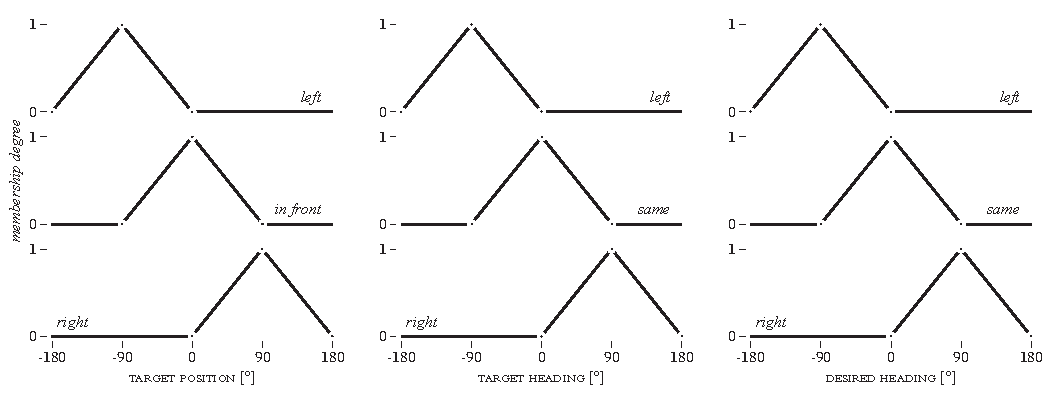
\includegraphics[width=\figurewidth]{scirep/si-predator_db}\\
  \scriptsize
  \vspace*{3mm}
  \begin{minipage}{\figurewidth}
    \textsc{r}1:\quad \textbf{if} (\textsc{target position} \textbf{is} \emph{right}) \textbf{then} (\textsc{desired heading} \textbf{is} \emph{right})\\
    \textsc{r}2:\quad \textbf{if} (\textsc{target position} \textbf{is} \emph{left}) \textbf{then} (\textsc{desired heading} \textbf{is} \emph{left}) \\
    \textsc{r}3:\quad \textbf{if} (\textsc{target position} \textbf{is} \emph{in front}) \textbf{and} (\textsc{target heading} is \emph{right}) \textbf{then} (\textsc{desired heading} \textbf{is} \emph{right})\\
    \textsc{r}4:\quad \textbf{if} (\textsc{target position} \textbf{is} \emph{in front}) \textbf{and} (\textsc{target heading} \textbf{is} \emph{left}) \textbf{then} (\textsc{desired heading} \textbf{is} \emph{left})\\
    \textsc{r}5:\quad \textbf{if} (\textsc{target position} \textbf{is} \emph{in front}) \textbf{and} (\textsc{target heading} \textbf{is} \emph{same}) \textbf{then} (\textsc{desired heading} \textbf{is} \emph{same})
  \end{minipage}
  \caption{The hand-tuned fuzzy knowledge base of the predator fuzzy-rule-based system.}
  \label{figure:predator}
\end{figure}

Let $d^{(i,j)}_t=\|\vec{r}^{(j)}_t-\vec{r}^{(i)}_t\|$ denote the distance between artificial animals $i$ and $j$ at time instant $t$ and $\uvec{d}^{(i,j)}_t=(\vec{r}^{(j)}_t-\vec{r}^{(i)}_t)/d^{(i,j)}_t$ the unit vector pointing from $i$ to $j$ at time instant $t$. The angular position of artificial animal $j$ with respect to $i$ is then
%
\begin{equation}
  \theta^{(i,j)}_t=\arccos\left(\uvec{v}^{(i)}_t \cdot \uvec{d}^{(i,j)}_t\right)
\end{equation}
%
and the relative orientation of artificial animal $j$ with respect to $i$
%
\begin{equation}
  \phi^{(i,j)}_t=\phi^{(j)}_t-\phi^{(i)}_t.
\end{equation}

Let $\kappa$ be a predator and $\alpha$ its current target. To compute the predator's desired heading its fuzzy-rule-based system input variables \textsc{target position} and \textsc{target heading} were set to $\theta^{(\kappa,\alpha)}_t$ and $\phi^{(\kappa,\alpha)}_t$, respectively.

The principal focus of the study was the analysis of the evolved behaviour when varying exposure to multiple simultaneous predation pressures. We used predators that according to previous research might pressure prey towards a) grouping \cite{biswas2014causes,kunz2006prey,olson2013predator,olson2016evolution} (\ie attack the most peripheral prey individual or attack the nearest prey individual) and b) dispersing \cite{olson2013predator} (\ie attack the most central prey individual or attack high density areas).

Let $\set{N}^{(i)}_t=\{j \in \set{I}|\ j \neq i, d^{(i,j)}_t \leq r^{(i)}_\textnormal{v}\}$ denote the neighbourhood of prey individual $i$. High density area attacking predators ($h$) detected and pursued the prey individual with the highest amount of nearby neighbours;
%
\begin{equation}
  \alpha^{(h)}_t = \argmax_{i \in \set{I}} \left|\set{N}^{(i)}_t\right|.
\end{equation}

Note that in the case of a high density area attacking predator (\HDAA predator) the targeted prey individual constantly changed, so that the \HDAA predator effectively detected and pursued the highest density area. Following Olson\etal \cite{olson2013predator} the \HDAA predators moved at a slower speed than prey and were also less manoeuvrable. If the \HDAA predator was close enough to any of the prey individuals (\ie $d^{(h,i)}_t\leq r^{(h)}_\textnormal{c},\ i \in \set{I}$) they were marked as captured. Note also that the \HDAA predator could consume any prey individual and not only the targeted prey individual, therefore mimicking predators capable of attacking and capturing several prey individuals in a single predation event \cite{goldbogen2011mechanics,nottestad1999herring,nottestad2002whales,mori2006first}.

Predators that attack the nearest, the most peripheral or the most central prey individual detect, pursue, attack and capture a single prey individual \cite{demsar2014simulated}. In this study we label them with the common name single-target attack or \ST predators. Note that in contrast to \HDAA predators, in the case of an \ST predator the target prey individual was detected only on special occasions and then pursued until captured or until the predator's hunt duration expired. The detection of the target prey individual occurred at the time instant when the \ST predator appeared or the currently targeted prey individual died during pursuit.

Following previous research \cite{demsar2014simulated,hemelrijk2000towards,hemelrijk2005construction,hildenbrandt2010selforganized}
%
\begin{equation}
  P^{(i)}_t = \frac{1}{\left|\set{N}^{(i)}_t\right|}\left\| \sum_{j \in \set{N}^{(i)}_t} \uvec{d}^{(i,j)}_t \right\|
  \label{equation:peripherality}
\end{equation}
%
is the peripherality of prey individual $i$ at time instant $t$. The peripherality of stragglers, prey individuals with no visible neighbour, \ie $\set{N}^{(i)}_t=\emptyset$, was set to $+\infty$. Let $s$ be an \ST predator. The nearest, $\alpha^{(s)}_\textnormal{n}$, the most peripheral, $\alpha^{(s)}_\textnormal{p}$, and the most central prey individual, $\alpha^{(s)}_\textnormal{c}$, were defined as
%
\begin{equation}
  \alpha^{(s)}_\textnormal{n} = \argmin_{i \in \set{I}} d^{(s,i)}_\sigma,
\end{equation}
%
\begin{equation}
  \alpha^{(s)}_\textnormal{c} = \argmin_{i \in \set{I}} P^{(i)}_\sigma,
\end{equation}
%
\begin{equation}
  \alpha^{(s)}_\textnormal{p} = \argmax_{i \in \set{I}} P^{(i)}_\sigma,
\end{equation}
%
where $\sigma$ is the time instant of target prey individual detection. In view of recent research by Biswas\etal, which suggests that prey clumping emerges regardless of predator confusion \cite{biswas2014causes}, when an \ST predator was close enough to its targeted prey individual (\ie $d^{(s,\alpha)}_t\leq r^{(s)}_\textnormal{c}$, where $\alpha$ is the currently targeted prey) the latter was marked as captured. Meaning that in contrast to previous research \cite{demsar2015simulating,kunz2006prey,olson2013predator,olson2016evolution}, the possibility of the predator getting confused was not explicitly modelled. In other words, predators in our model did not change their target and remained focused throughout the whole hunt event. As a contrast to \HDAA predators, \ST predators were faster than prey, but were also less manoeuvrable.

%-----
\subsection{Prey}

Every prey individual's behaviour was governed by its own fuzzy-rule-based system that, by the application of fuzzy reasoning over an evolving set of if-then rules, determined the individual's desired heading in the next time step. Only the fuzzy rule base was evolved; the fuzzy data base was kept constant (see \figurename~\ref{figure:prey}). The input variables can be decomposed into three parts: a) information regarding the living area, b) information regarding the nearest predator, and c) information regarding the interacting neighbour.

\begin{figure}
  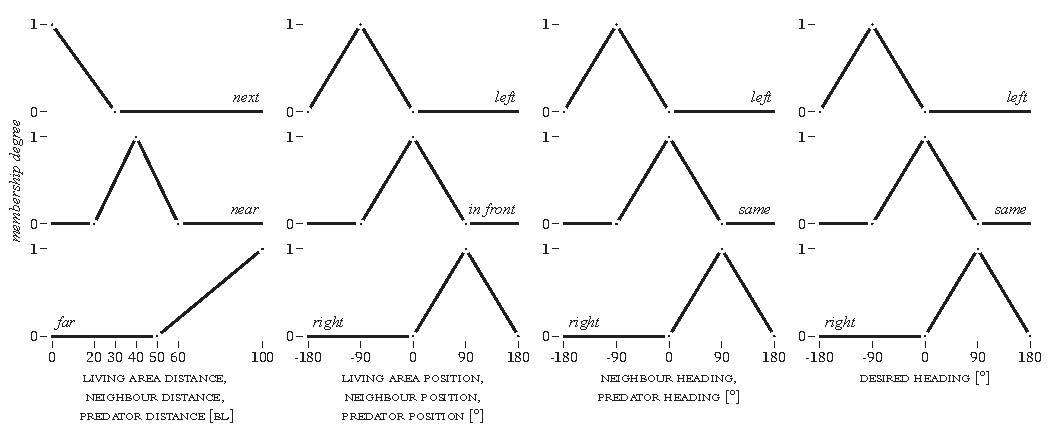
\includegraphics[width=\figurewidth]{scirep/si-prey_db}
  \caption{The data base for prey individuals. The rule base for prey individuals was generated using genetic fuzzy systems.}
  \label{figure:prey}
\end{figure}

At all times prey individuals were aware of the distance and angular position of the nearest point on the border of the living area (\figurename~\ref{figure:preyInput}a), so the input variables \textsc{living area distance} and \textsc{living area position} of prey individual $i$ were set to
%
\begin{equation}
  d^{(i)}_t=\min(0,\ \max(r_\textnormal{LA}-\|\vec{r}^{(i)}_t\|),\ r^{(i)}_\textnormal{v})
\end{equation}
%
and
%
\begin{equation}
  \theta^{(i)}_t=\arccos\left(\uvec{v}^{(i)}_t \cdot \uvec{r}^{(i)}_t\right),
\end{equation}
%
respectively.

\begin{figure}
  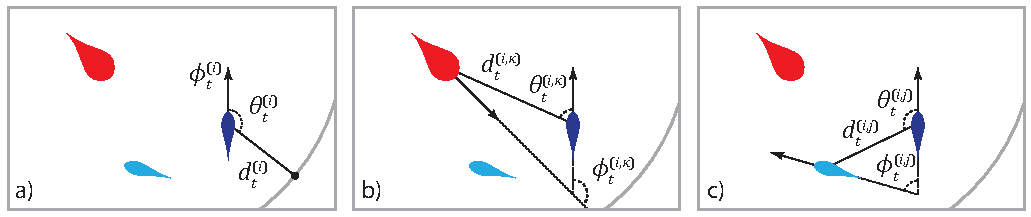
\includegraphics[width=\figurewidth]{scirep/si-interaction}
  \infigurecaption{a) distance, $d^{(i)}_t$, and angular position $\theta^{(i)}_t$ of the nearest point on the border of the living area, b) distance, $d^{(i,\kappa)}_t$, angular position, $\theta^{(i,\kappa)}_t$, and relative orientation, $\phi^{(i,\kappa)}_t$, of the nearest predator, c) distance, $d^{(i,j)}_t$, angular position, $\theta^{(i,j)}_t$, and relative orientation, $\phi^{(i,j)}_t$, of the interacting neighbour.}
  \caption{Quantities available to prey individuals in order to determine their desired heading.}
  \label{figure:preyInput}
\end{figure}

As empirical data suggests that animals in groups usually react to predator attacks\cite{partridge1982structure,pitcher1983predator}, it is safe to assume that in most cases prey individuals can detect the incoming predator attack at some point in time. For this reason, in our model, prey individuals were aware of the nearest visible predator. From the prey individual's point of view this is the predator that poses the highest threat \cite{rieucau2014experimental}. The input variables \textsc{predator distance}, \textsc{predator position}, and \textsc{predator heading} were set to $d^{(i,\kappa)}_t$, $\theta^{(i,\kappa)}_t$, and $\phi^{(i,\kappa)}_t$, respectively (\figurename~\ref{figure:preyInput}b). Here $\kappa$ denotes the nearest currently visible predator of prey individual $i$, computed as
%
\begin{equation}
  \kappa = \argmin_{k \in \set{K}} d^{(i,k)}_t,\ \set{K}=\{k \in \set{S} \cup \set{H}|\ d^{(i,k)}_t \leq r^{(i)}_\textnormal{v}\},
\end{equation}
%
where $\set{K}$ is the set of predators (\ST or \HDAA) currently visible by prey individual $i$. If the prey individual did not see any predators the input variables were marked as \textsc{undefined}. If-then rules with any of their input variables marked as \textsc{undefined} were excluded from fuzzy reasoning.

A large-scale empirical study conducted in Rome \cite{ballerini2008interaction} discovered an anisotropic nature of interactions in starling flocks. This type of interaction became known as topological interaction, where an individual interacts with $\approx$\num{6.5} of its nearest neighbours. Bode\etal \cite{bode2010perceived} proposed a much simpler interaction model capable of replicating the anisotropic nature of the interactions observed in the empirical study. In their model interaction is stochastic in nature and the probability of prey individual $i$ interacting with prey individual $j$ depends on visibility of individual $j$ and is inversely proportional to its distance,
%
\begin{equation}
  p(i,j) = \begin{cases}
    \frac{1}{d^{(i,j)}_t}, &\text{iff }j \in \set{N}^{(i)}_t\\
    0, &\text{otherwise}.
  \end{cases}
  \label{equation:neigbour}
\end{equation}

Following Bode\etal \cite{bode2010perceived} prey individuals in our model at every time instant interacted with only one other prey individual, as this greatly reduces the number of fuzzy-rules that have to be evaluated per prey individual. The fuzzy-rule-based system input variables \textsc{neighbour distance}, \textsc{neighbour position}, and \textsc{neighbour heading} were set to $d^{(i,j)}_t$, $\theta^{(i,j)}_t$, and $\phi^{(i,j)}_t$, respectively (\figurename~\ref{figure:preyInput}c). Like in the case of the input variables related to the nearest predator, if the prey individual had no visible neighbour, i.e $\set{N}^{(i)}_t = \emptyset$ in \eq \eqref{equation:neigbour}, the input variables were marked as \textsc{undefined}.

Evolution was achieved by the application of genetic algorithms over the fuzzy-rule-based systems, \ie by genetic fuzzy systems. Genetic fuzzy systems have been extensively used for the optimization of hand-crafted fuzzy knowledge bases, and evolution of data bases, rule bases or the whole fuzzy knowledge base \cite{cordon2004ten,fernandez2015revisiting,herrera2008genetic}. In our case we pre-specified the data base and used a genetic fuzzy system to evolve only the rule bases of every prey individual. Our inspiration were messy genetic algorithms \cite{goldberg1989messy} which use the Pittsburgh approach: each individual in the population is a complete rule base \cite{hoffman1997evolutionary,smith1980learning}.

\begin{table}
  \caption{Parameters of the genetic fuzzy system.}
  \label{table:ga}
  \begin{tabular}{l l}
    \toprule
    Description & Default (tested) value \\ [0.5ex]
    \midrule
    Number of if-then rules per individual & 2--30 (2--50) \\
    Number of antecedents per rule & 1--2 (1--3) \\
    Mutation rate & 2\% \\
    Mutation intensity & 3 \\
    \bottomrule
  \end{tabular}
\end{table}

The initial population of prey individuals had a randomly generated rule base. The only constraints were the number of if-then rules per individual and the number of antecedents per rule (see \tablename~\ref{table:ga}). The constraints were selected to keep an individual's reasoning as simple as possible. Preliminary tests of the influence of these two constraints on the resulting behaviour by performing evolutions with a higher maximal number of rules (50) and/or antecedents (3) showed results similar to those reported in the main article.

When a prey individual died a new prey individual (child) was created by merging the rule bases of two prey individuals (parents) that were still alive. Selection of parents was fitness proportionate, where the fitness was based on the prey individual's energy level. The number of rules in the rule base of the child prey individual was a uniformly distributed random number between the number of rules in the parent's rule base, whose rule base had the lowest number of rules, and the number of rules in the other parent's rule base. For example, if the rule base of one parent had 15 rules and the other 18 the child could have anywhere between 15 and 18 rules.

Rules in the rule bases of the two parents that had the same antecedent part and the same consequent part of the if-then rule were treated as equal. First equal rules were copied to the child's rule base. Following that the remaining slots were filled with random rules from the set of non-equal rules. Once the child's rule base had the required number of rules there was a 2\% chance a mutation could trigger (mutation rate). There were two kinds of mutations in our genetic fuzzy system; the first type inserted new random rules into the child's rule base, the other removed existing rules. The amount of rules inserted or removed was a uniformly distributed random number between 1 and 3 (mutation intensity). Note that each mutation type could trigger independently so every time a new child prey individual was created each mutation type (insert rules, remove rules) had a 2\% chance of triggering.

%-----
\subsection{Biological relevance of the parameters}

Where possible we attempted to set the model's parameters to biologically relevant values (see \tablename~\ref{table:parameters:SM}). We modelled the prey species after the Pacific Blue-eye (\emph{Pseudomugil signifier}), a fish species that is well known for schooling \cite{herbertread2010sensory,herbertread2015intiation,herbertread2016threedimensional}. In the case of Herbert-Read\etal \cite{herbertread2015intiation} the body lengths (\si{\bodylength}) of captured Pacific Blue-eyes were from \SIrange{2}{3}{\cm}. Other studies \cite{pusey2004freshwater} report an average \si{\bodylength} of approximately \SI{3.5}{\cm}. In our case we used a body length value of \SI{3}{\cm}. The cruising speed of Pacific Blue-eyes is approximately \mps{0.124} $\approx$ \BLps{4} \cite{herbertread2015intiation}. For prey visibility distance we used the equation provided by Tyrell\etal \cite{tyrrell2013looking}. We could not find the exact spatial resolving power of the Pacific Blue-eye so we used the value of a fish of similar size, the zebrafish (\emph{Danio rerio}) \cite{pita2015vision}. This value is relevant since fish of similar size, have similar sized retinas, and thus similar vision capabilities \cite{hairston1982fish}. The zebrafish can spot an object of size \SI{3}{\cm} (the size of a prey individual in our model) at a distance of \SI{330}{\cm}. Because the zebrafish is slightly larger than the Pacific Blue-eye and fish with larger retinas can see farther \cite{hairston1982fish}, we set the visibility distance of prey individuals to \BL{100}. As pointed out by Domenici \cite{domenici2001scaling}, speed changes and body size play a major role in turning rates of fish. Because the speed in our model is constant we could not use the empirical data about fish turning rates. Which is why the maximum manoeuvrability of prey individuals was tuned by hand in such a way that with a hand-tuned fuzzy-rule-based system prey individuals were able to avoid others effectively but without introducing too erratic or jerky movements.

An example of a single-target attack predator that attacks schools of Pacific Blue-eyes is the flathead Gudgeon (\emph{Philypnodon grandiceps}) \cite{herbertread2016threedimensional}. The flathead Gudgeon is usually around \SI{8}{\cm} in length, but it can sometimes grow up to \SI{12}{\cm} in length \cite{pusey2004freshwater}, so we set the size of \ST predators in our model to \BL{3} (\SI{9}{\cm}). The linear regression formula provided by Domenici \cite{domenici2001scaling} suggests that a predator that is 3 times larger than the prey is also approximately \num{1.4} times faster than the prey. Based on that we set the speed of \ST predators in our model to \BLps{5.6}. The \ST predator vision radius calculated using the same approach as for prey individual's \cite{hairston1982fish,pita2015vision,tyrrell2013looking}, would be approximately \BL{300}. However, in mammals \cite{veilleux2014visual}, once the effects of eye size and phylogeny have been statistically controlled, predatory habits are associated with a higher visual acuity. In addition, some aquatic predators, \eg swordfish (\emph{Xiphias gladius}), warm their retina to significantly improve temporal resolution, and hence the detection of rapid motion \cite{fritsches2005warm}. Since the goal of this research is the investigation of behaviour that evolves under various predation pressure mixtures, we wanted to guarantee that the predators can always find and target the most vulnerable prey individual (with respect to the predator's predation tactic). Which is why the vision of predators in our model is not limited. With this we also removed the occurrences when the predator ``did not see a potential prey target.'' To calculate the manoeuvrability of \ST predators we used the equation designed on empirical data by McKenzie\etal \cite{mckenzie2007locomotion}. Using this equation, we calculated that a single target predator should be \num{1.7} times less manoeuvrable than prey.

\begin{table}
  \caption{The individual based model's parameters; \ST -- single-target attack, \HDAA -- high density area attack.}
  \label{table:parameters:SM}
  \renewcommand*{\arraystretch}{.99} % reduce interline spacing by 1%; resolves "Float too large for page by 1.35126pt"
  \begin{tabular}{l l l}
    \toprule
    Parameter & Description & Default value \\
    \midrule
    $\tau$ & Update step & \SI{1}{\second} \\
    $\si{\bodylength}$ & Body length & \SI{3}{\cm} \\
    $r_\textnormal{LA}$ & Living area radius & \BL{350} \\
    \midrule
    $\set{I}$ & Set of prey individuals (size) & 100 \\
    $b^{(i)}$ & Prey appearance area radius & \BL{325} \\
    $s^{(i)}$ & Prey size & \BL{1} \\
    $v^{(i)}$ & Prey speed & \BLps{4} \\
    $r^{(i)}_\textnormal{v}$ & Prey vision radius & \BL{100} \\
    $\omega^{(i)}_\textnormal{max}$ & Prey maximum manoeuvrability &  \rps{0.23}\\
    $\epsilon_0$ & Prey initial energy & \num{1000} \\
    $\epsilon_\textnormal{l}$ & Prey living energy gain & 1 \\
    $\epsilon_\textnormal{c}$ & Prey collision penalty & \num{-10} \\
    $\epsilon_\textnormal{w}$ & Prey wandering penalty & \num{-10} \\
    \midrule
    $t_\textnormal{r}$ & Predator re-appearance time & \SIrange{600}{1200}{\second} \\
    $t_\textnormal{h}$ & Predator hunt duration & \SI{600}{\second} \\
    \hdashline
    $\set{S}$ & Set of \ST predators (size) & 0--8 \\
    $b^{(s)}$ & \ST predator appearance distance & \BL{400} \\
    $s^{(s)}$ & \ST predator size & \BL{3} \\
    $v^{(s)}$ & \ST predator speed & \BLps{5.6} \\
    $r^{(s)}_\textnormal{c}$ & \ST predator catch distance & \BL{3} \\
    $\omega^{(s)}_\textnormal{max}$ & \ST predator maximum manoeuvrability & \rps{0.16} \\
    \hdashline
    $\set{H}$ & Set of \HDAA predators (size) & 0--8 \\
    $b^{(h)}$ & \HDAA predator appearance distance & \BL{400} \\
    $s^{(h)}$ & \HDAA predator size & \BL{12} \\
    $v^{(h)}$ & \HDAA predator speed & \BLps{3} \\
    $r^{(h)}_\textnormal{c}$ & \HDAA predator catch distance & \BL{12} \\
    $\omega^{(h)}_\textnormal{max}$ & \HDAA predator maximum manoeuvrability & \rps{0.03} \\
    \midrule
    $E$ & Duration of evolution & \SI{10000000}{\second} \\
    $I$ & Number of iterations & 20 \\
    \bottomrule
  \end{tabular}
\end{table}

\begin{largefigure} % float too large for page by 16pt [with largefigure environment the max is 37pt]
  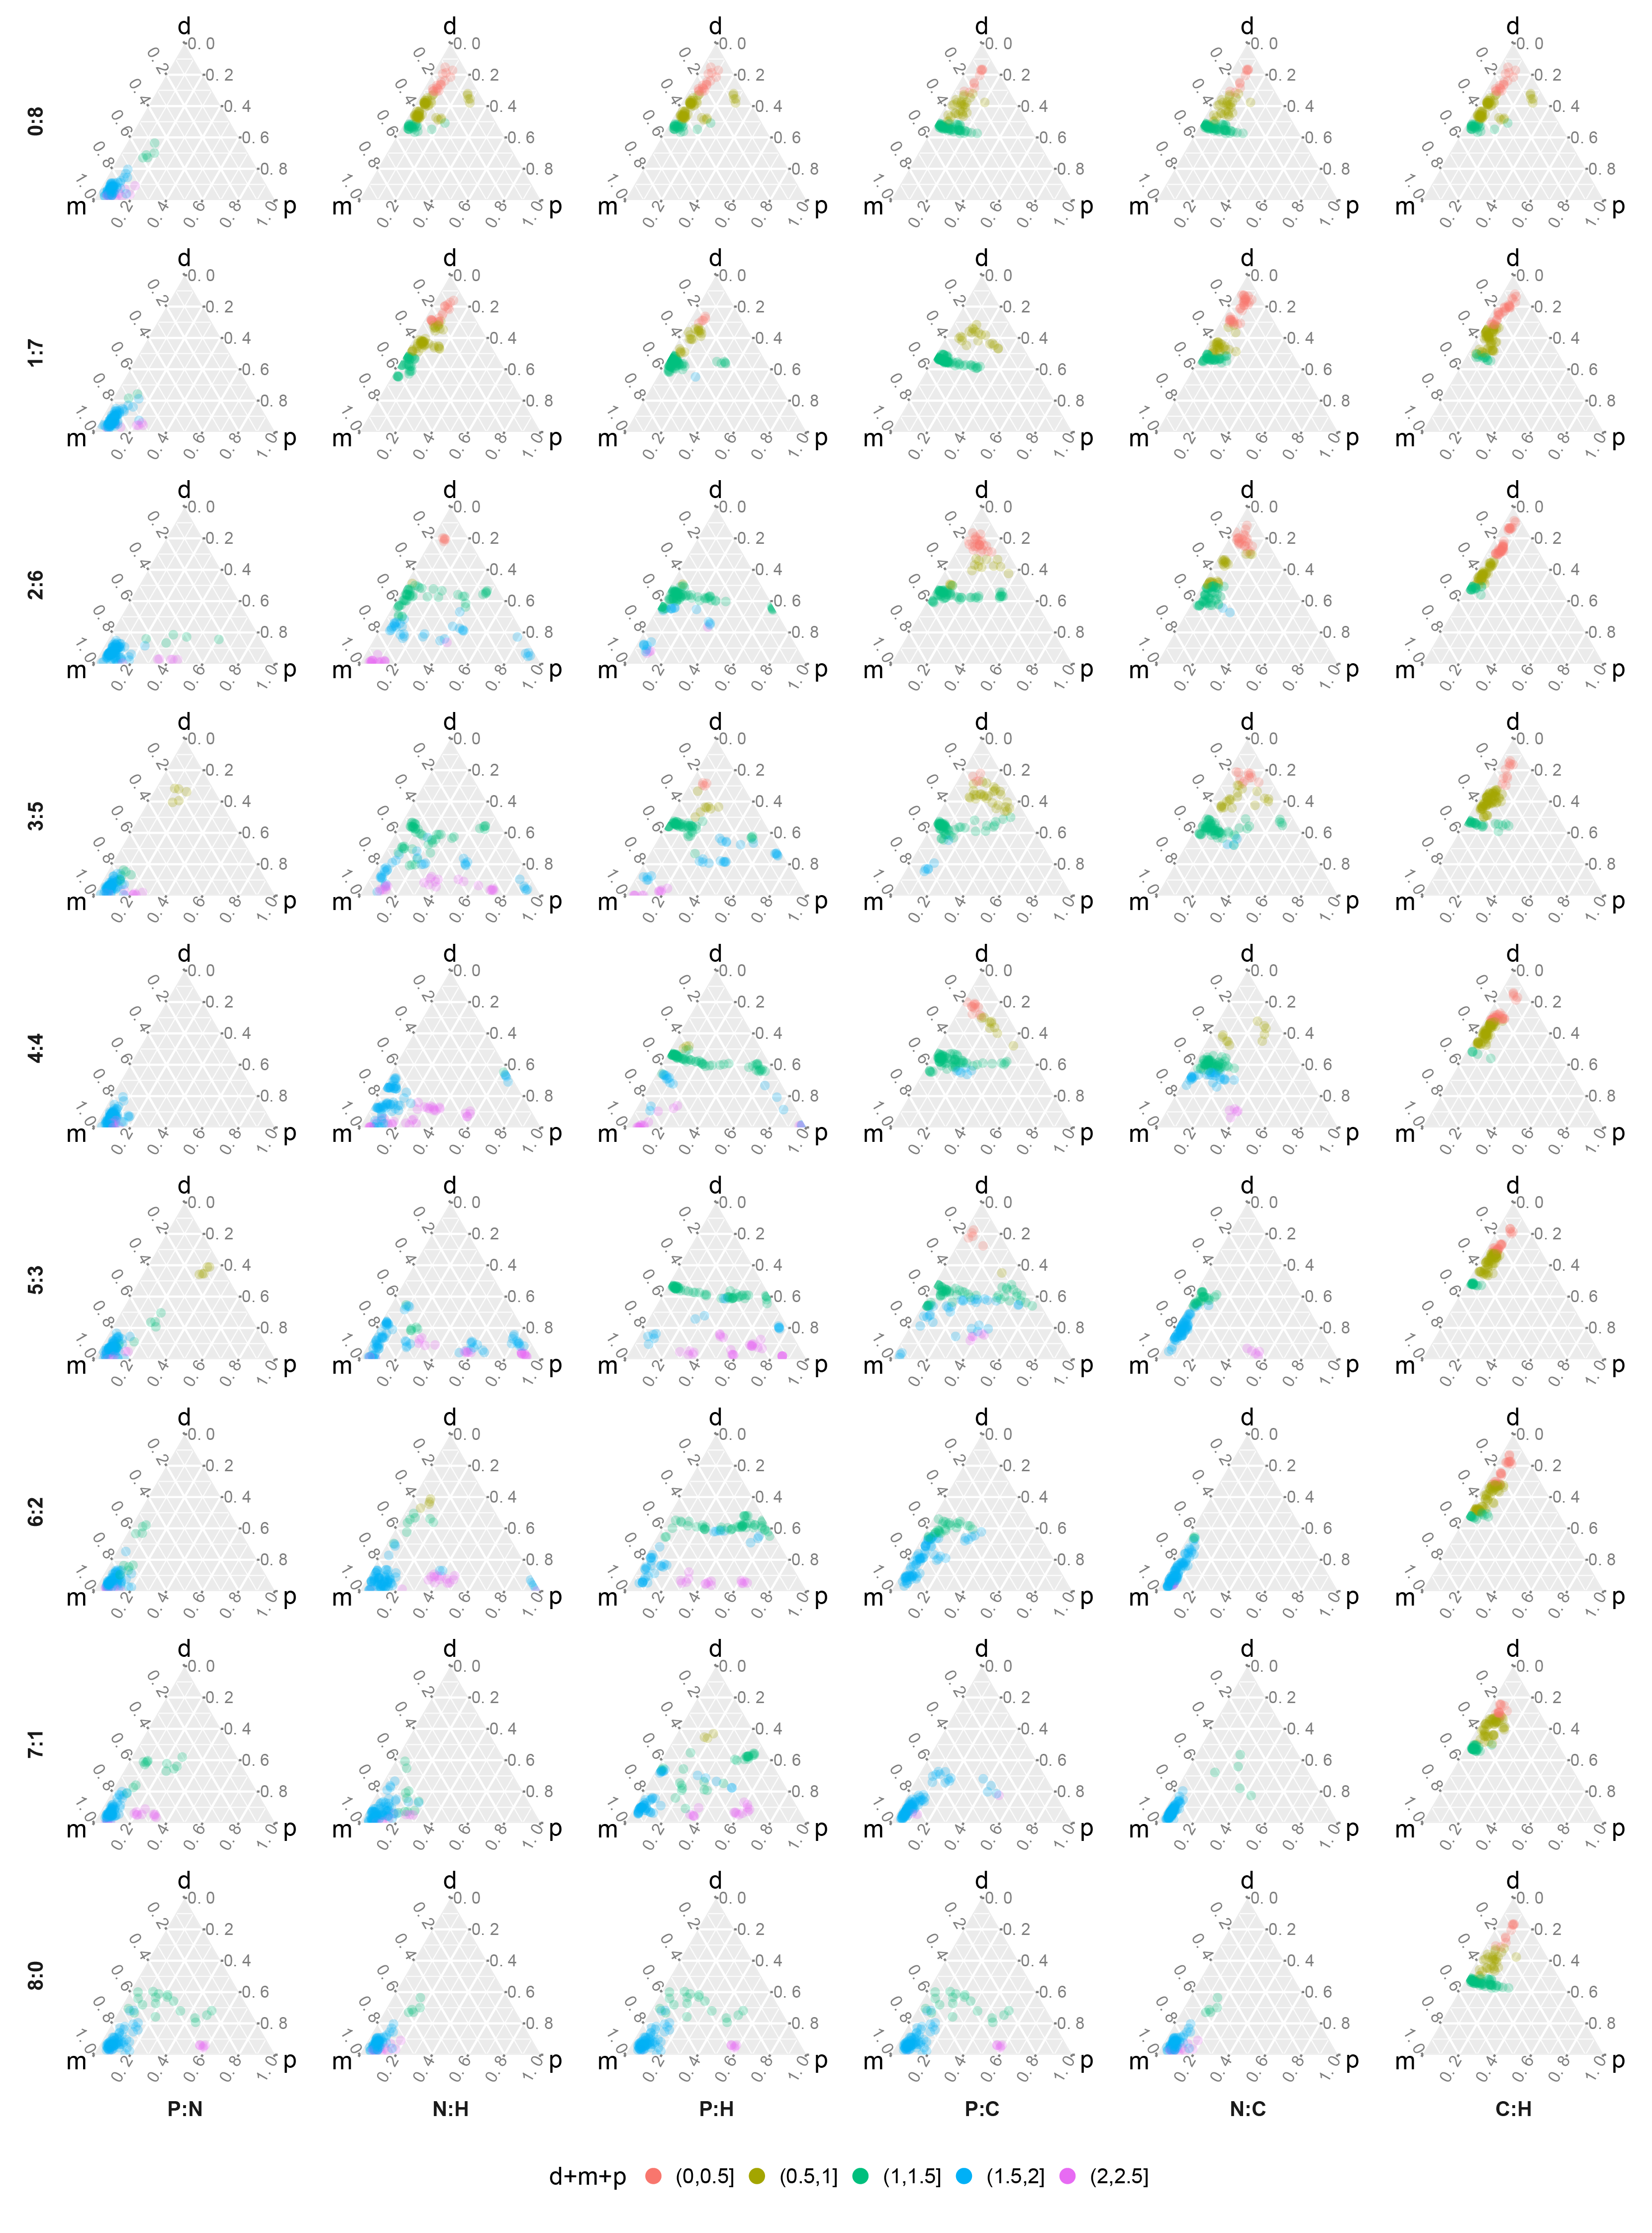
\includegraphics[width=\figurewidth]{scirep/si-tern}
  \infigurecaption{P -- attack prey individuals located at the periphery of the prey groups, N -- attack the nearest prey individual, C -- attack the most central prey individual in a prey group, and H -- high density area attacks. The predator pressure combinations and mixtures were ordered so that the top row and left column, represent the highest pressure towards grouping, the right column and bottom row the highest pressure towards dispersing. The middle section represents antagonistic predation pressures. The scales of the ternary plot were arranged so that the top corner indicates low density, the bottom left corner indicates high density and angular momentum, and the bottom right corner indicates high density and polarization. Note that the ternary plot shows the relationship between the three variables (\ie which one dominates, in relative terms). Since the same point can represent completely different behaviours the sum of the three dimensions is used for colour coding.}
  \caption{Normalized prey density (d), polarization (p) and angular momentum (m) for all predation pressure mixtures, N=\num{5400}.}
  \label{figure:antagonistic:SM}
\end{largefigure}

\begin{video}
  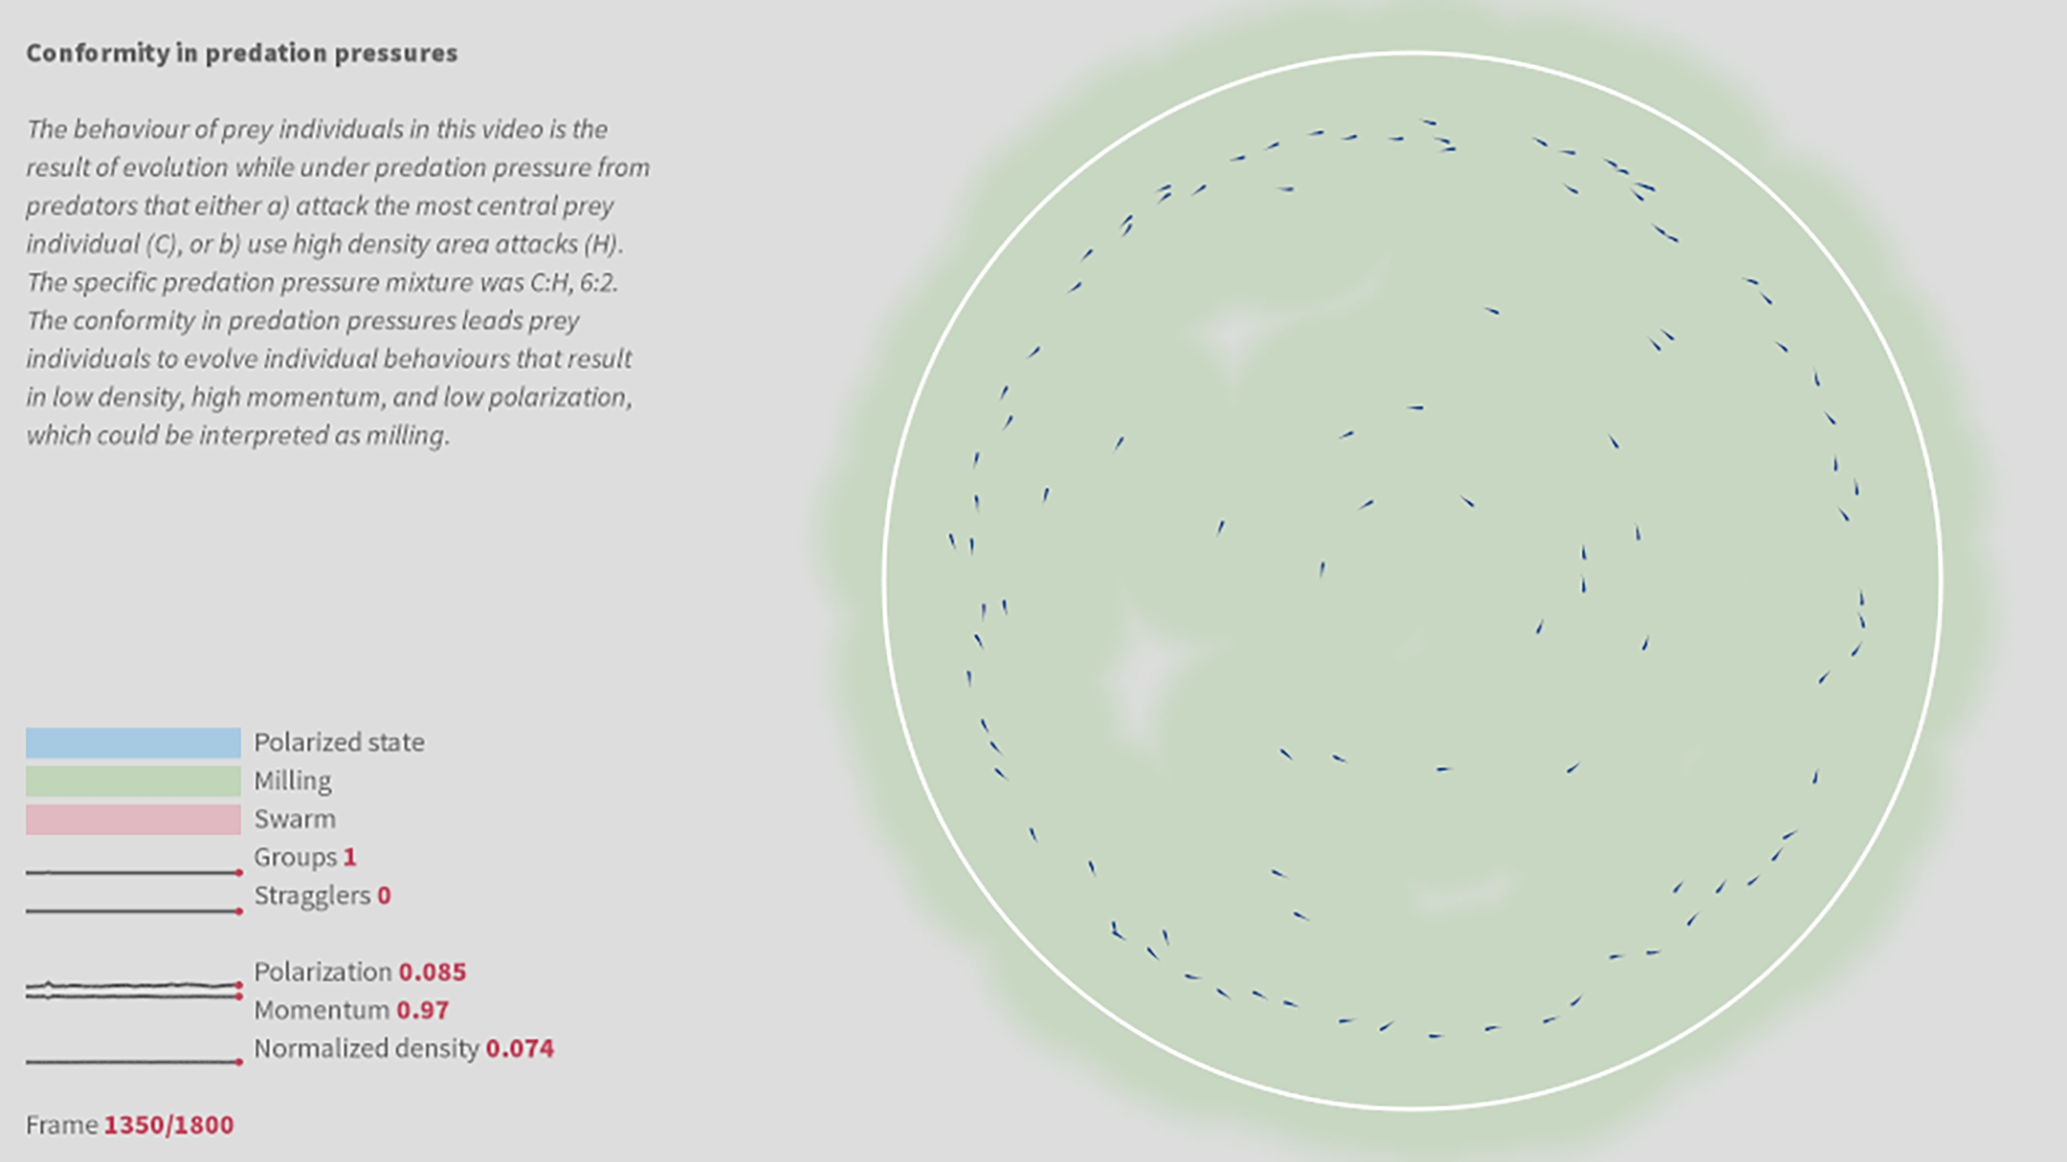
\includegraphics[width=\figurewidth]{scirep/si-V1_1350}
  \infigurecaption{The behaviour of prey individuals in this video is the result of evolution while under predation pressure from predators that either a) attack the most central prey individual (C), or b) use high density area attacks (H). The specific predation pressure mixture was C:H, 6:2. The conformity in predation pressures leads prey individuals to evolve individual behaviours that result in low density, high momentum, and low polarization, which could be interpreted as milling.}
  \caption{Conformity in predation pressures.}
  \label{video:V1}
\end{video}

\begin{video}
  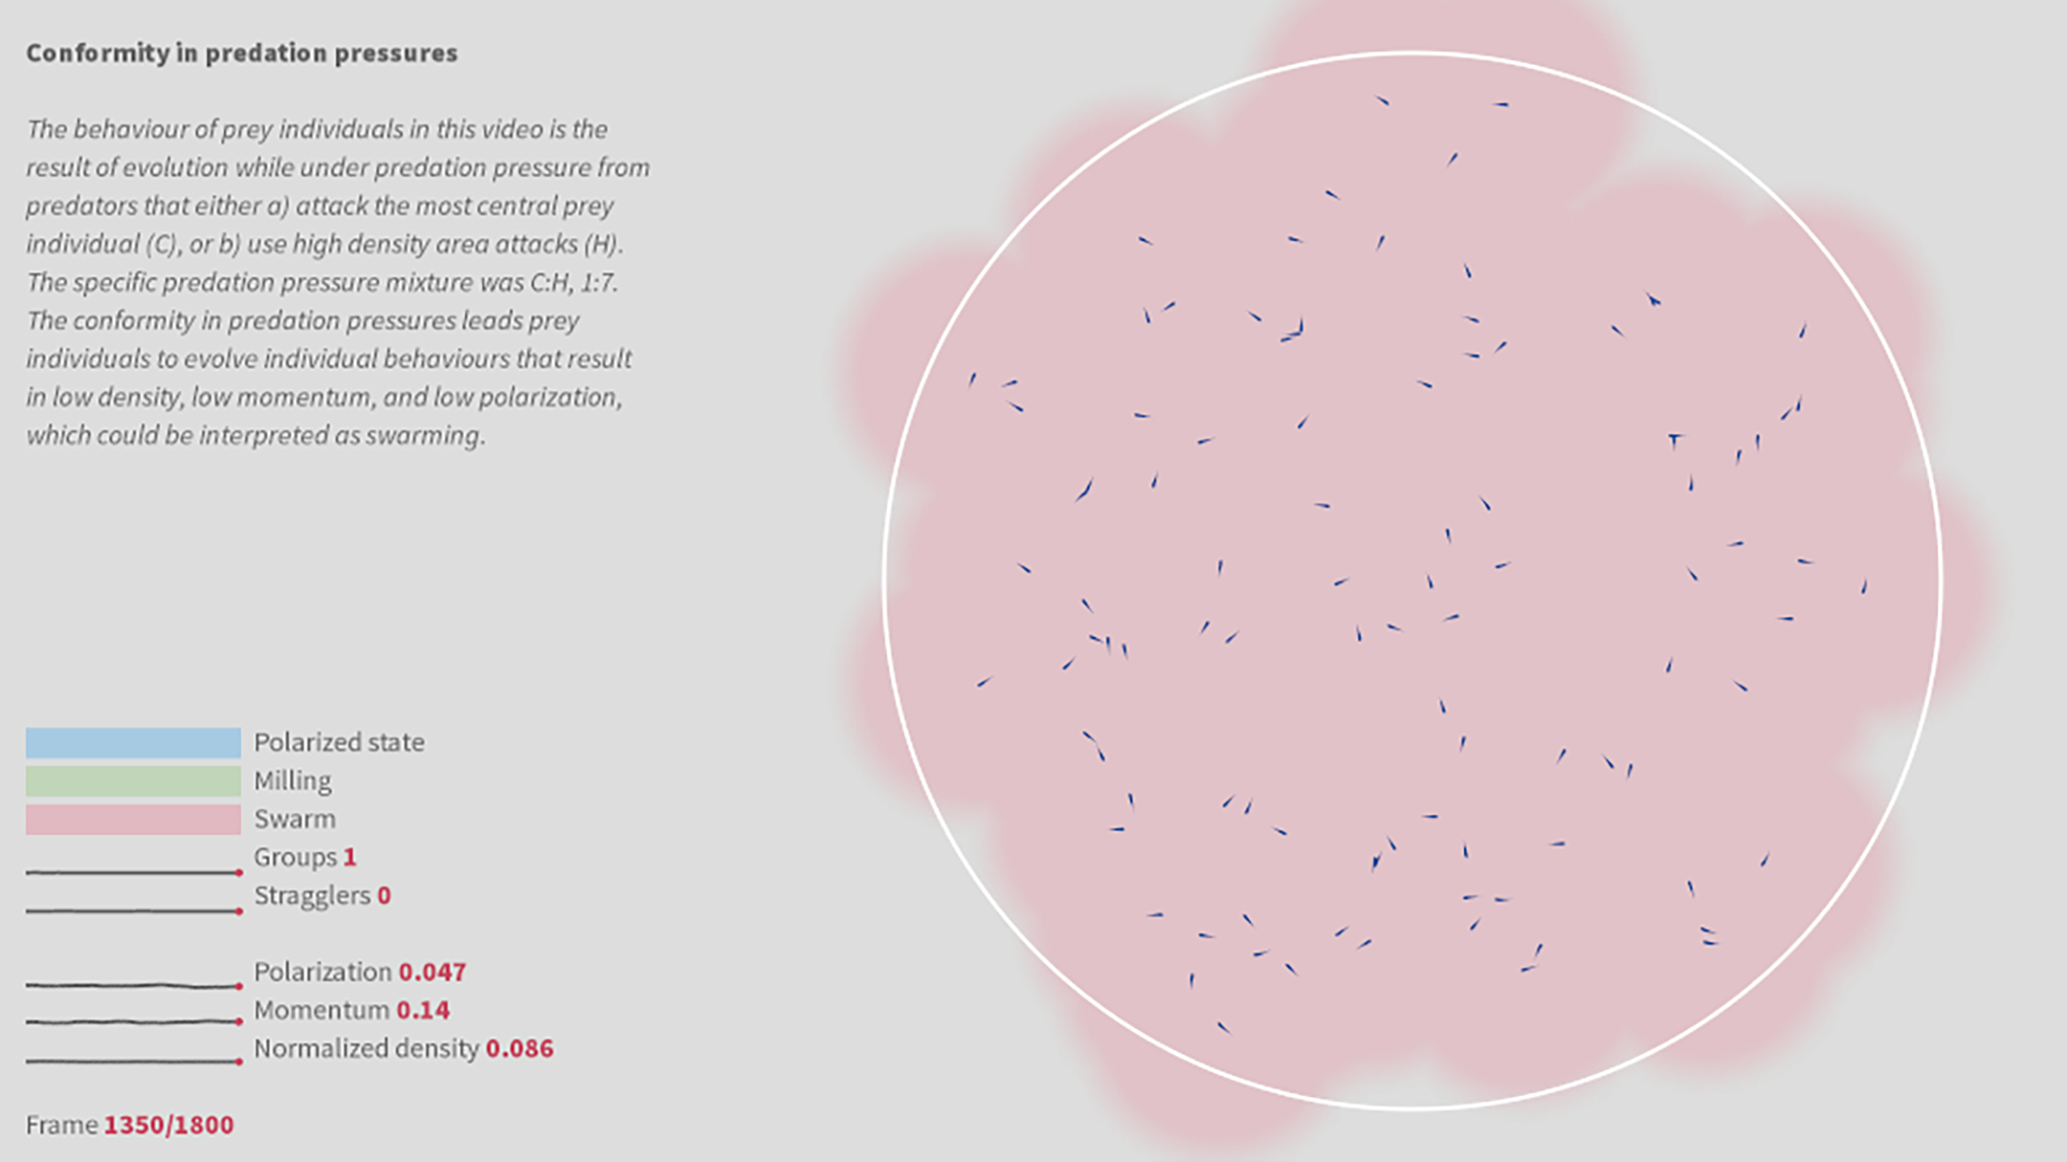
\includegraphics[width=\figurewidth]{scirep/si-V2_1350}
  \infigurecaption{The behaviour of prey individuals in this video is the result of evolution while under predation pressure from predators that either a) attack the most central prey individual (C), or b) use high density area attacks (H). The specific predation pressure mixture was C:H, 1:7. The conformity in predation pressures leads prey individuals to evolve individual behaviours that result in low density, low momentum, and low polarization, which could be interpreted as swarming.}
  \caption{Conformity in predation pressures.}
  \label{video:V2}
\end{video}

\begin{video}
  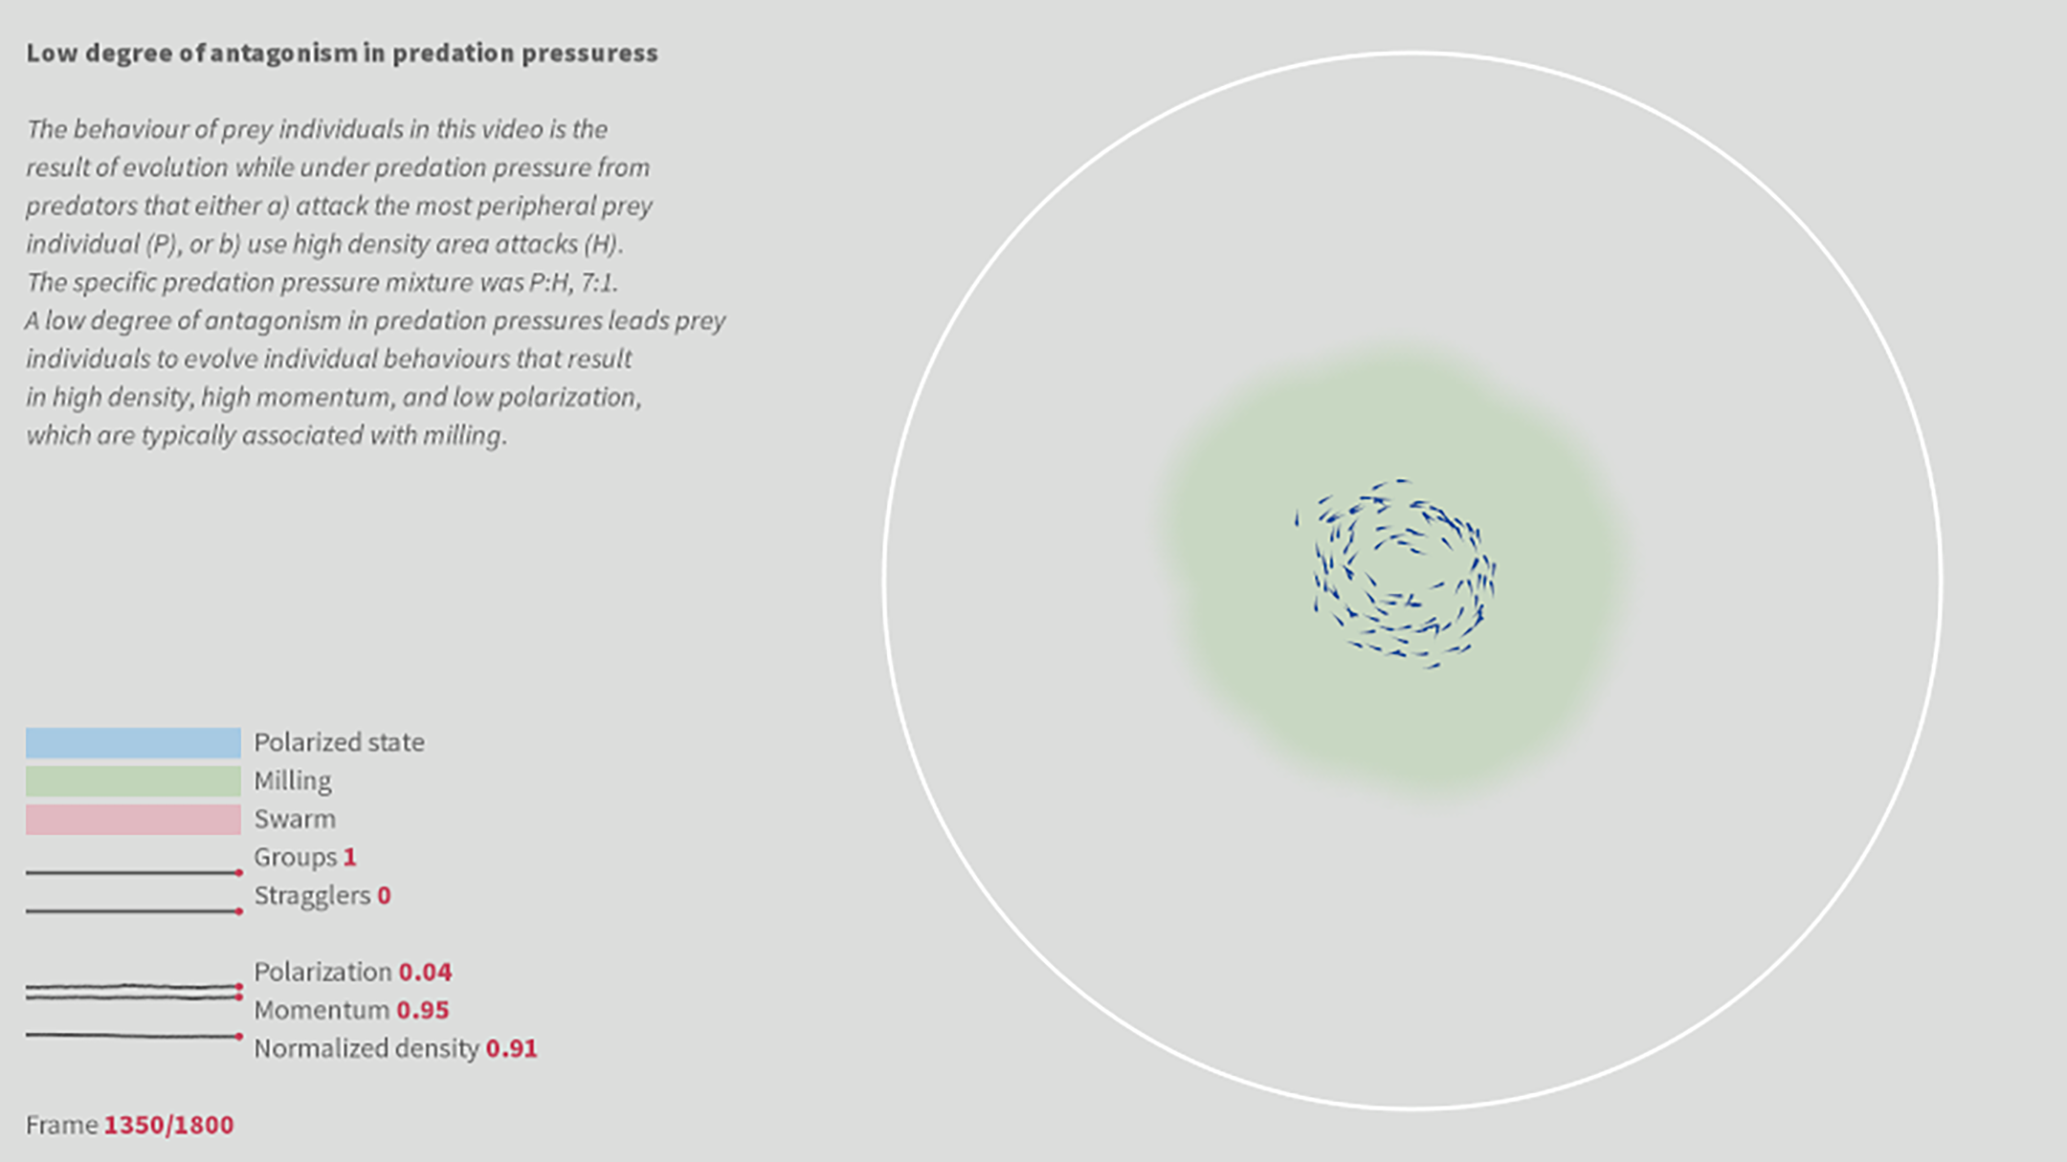
\includegraphics[width=\figurewidth]{scirep/si-V3_1350}
  \infigurecaption{The behaviour of prey individuals in this video is the result of evolution while under predation pressure from predators that either a) attack the most peripheral prey individual (P), or b) use high density area attacks (H). The specific predation pressure mixture was P:H, 7:1. A low degree of antagonism in predation pressures leads prey individuals to evolve individual behaviours that result in high density, high momentum, and low polarization, which are typically associated with milling.}
  \caption{Low degree of antagonism in predation pressures.}
  \label{video:V3}
\end{video}

\begin{video}
  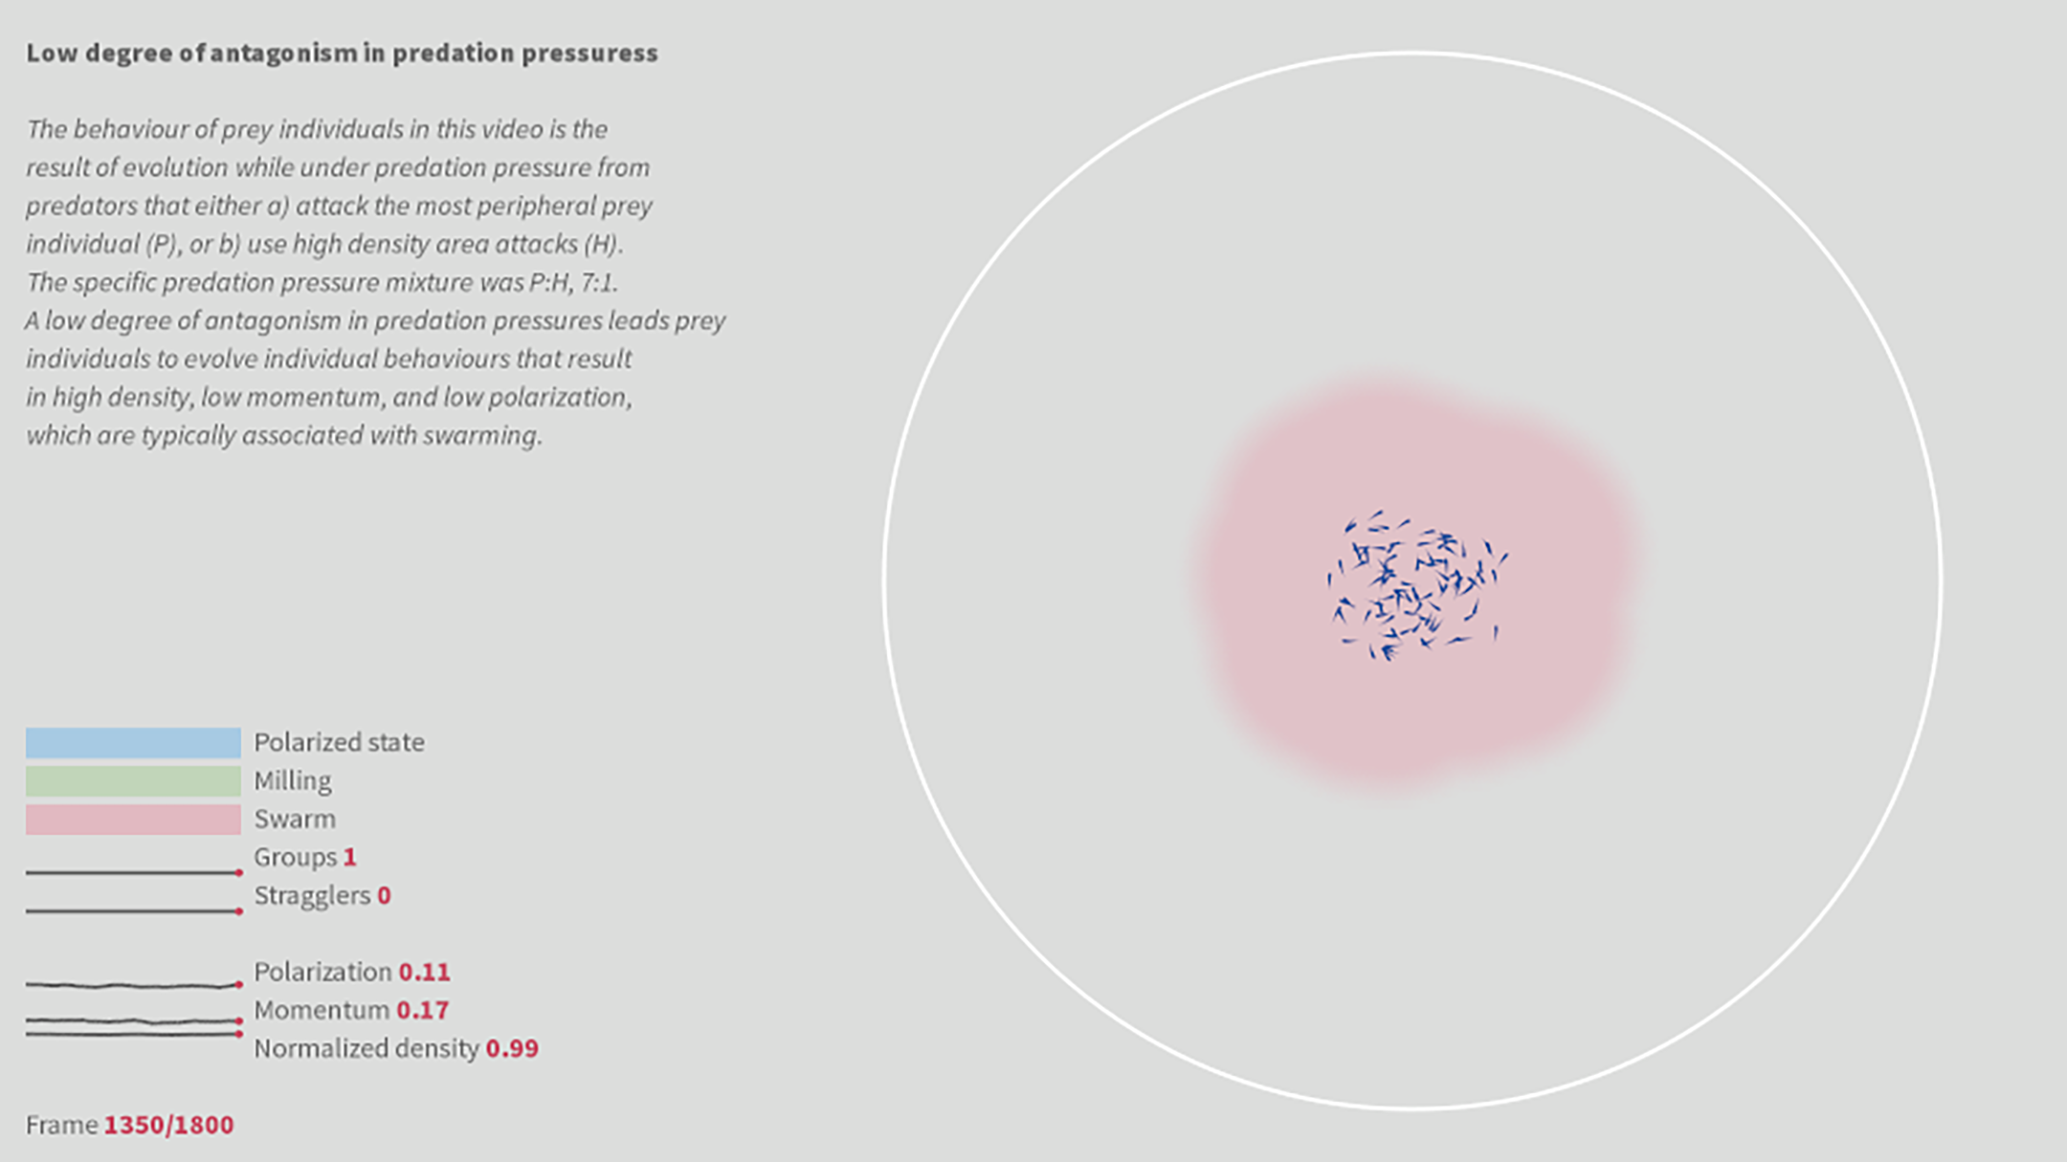
\includegraphics[width=\figurewidth]{scirep/si-V4_1350}
  \infigurecaption{The behaviour of prey individuals in this video is the result of evolution while under predation pressure from predators that either a) attack the most peripheral prey individual (P), or b) use high density area attacks (H). The specific predation pressure mixture was P:H, 7:1. A low degree of antagonism in predation pressures leads prey individuals to evolve individual behaviours that result in high density, low momentum, and low polarization, which are typically associated with swarming.}
  \caption{Low degree of antagonism in predation pressures.}
  \label{video:V4}
\end{video}

\begin{video}
  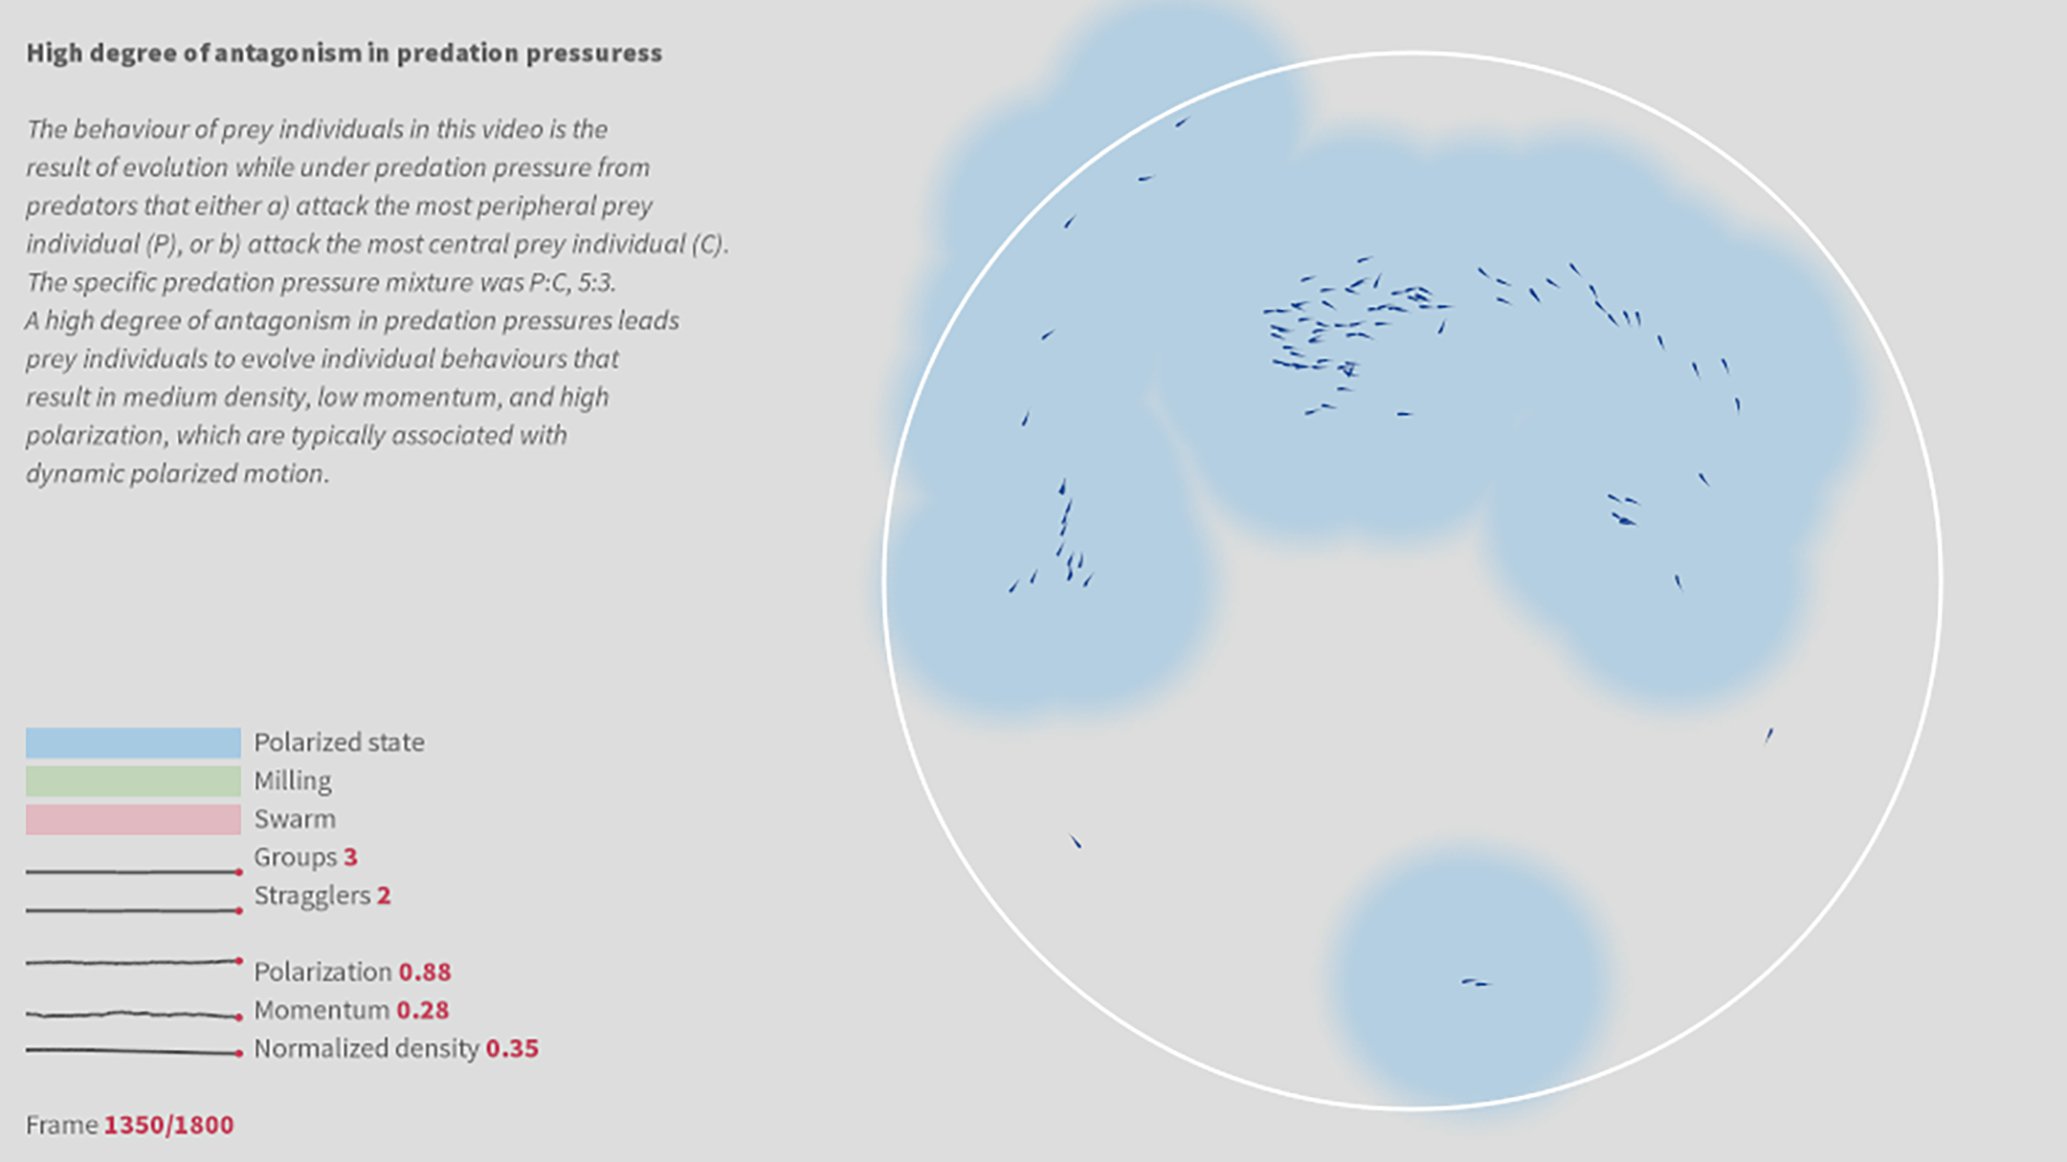
\includegraphics[width=\figurewidth]{scirep/si-V5_1350}
  \infigurecaption{The behaviour of prey individuals in this video is the result of evolution while under predation pressure from predators that either a) attack the most peripheral prey individual (P), or b) attack the most central prey individual (C). The specific predation pressure mixture was P:C, 5:3. A high degree of antagonism in predation pressures leads prey individuals to evolve individual behaviours that result in medium density, low momentum, and high polarization, which are typically associated with dynamic polarized motion.}
  \caption{High degree of antagonism in predation pressures.}
  \label{video:V5}
\end{video}

\begin{video}
  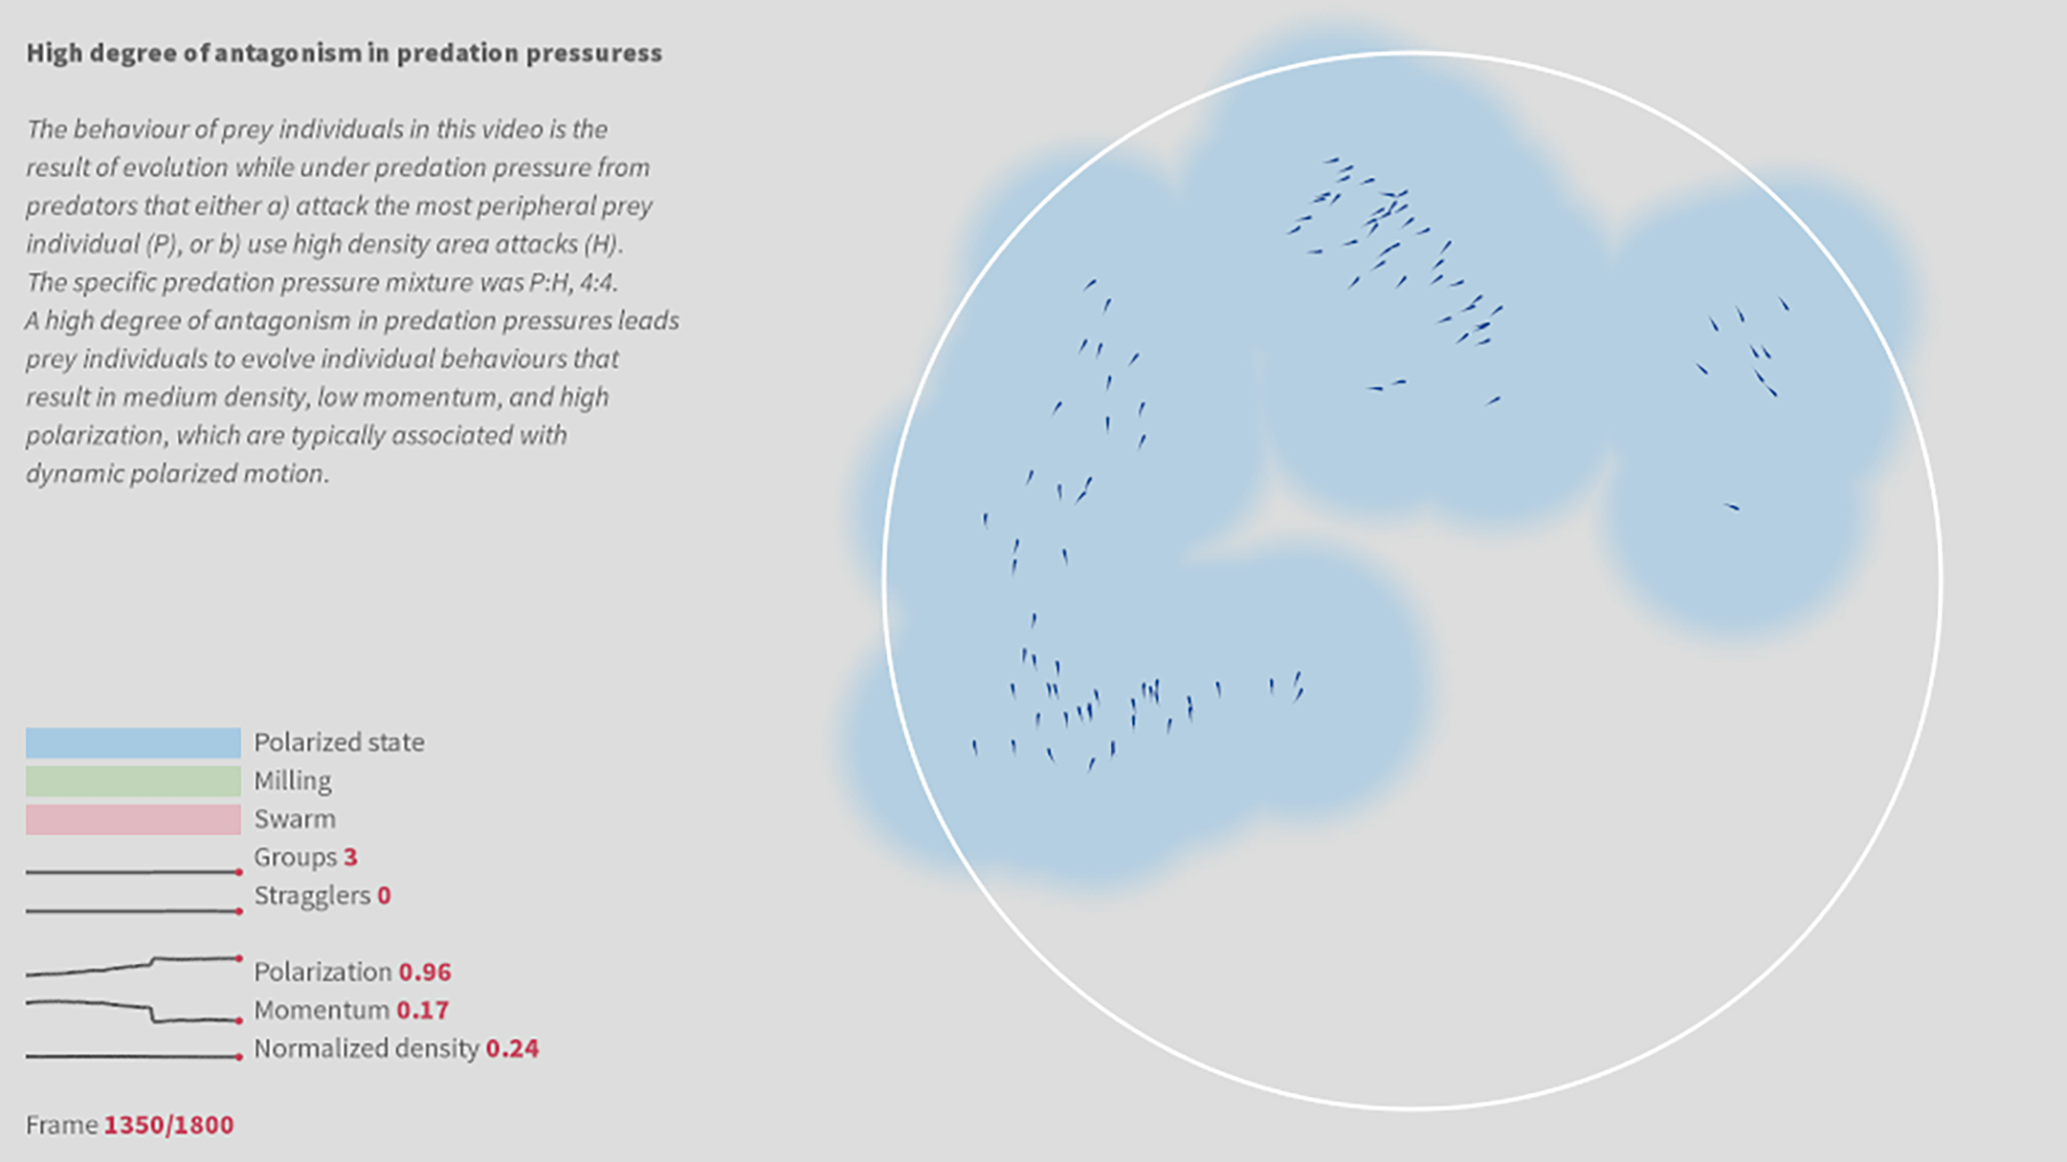
\includegraphics[width=\figurewidth]{scirep/si-V6_1350}
  \infigurecaption{The behaviour of prey individuals in this video is the result of evolution while under predation pressure from predators that either a) attack the most peripheral prey individual (P), or b) use high density area attacks (H). The specific predation pressure mixture was P:H, 4:4. A high degree of antagonism in predation pressures leads prey individuals to evolve individual behaviours that result in medium density, low momentum, and high polarization, which are typically associated with dynamic polarized motion.}
  \caption{High degree of antagonism in predation pressures.}
  \label{video:V6}
\end{video}

\begin{video}
  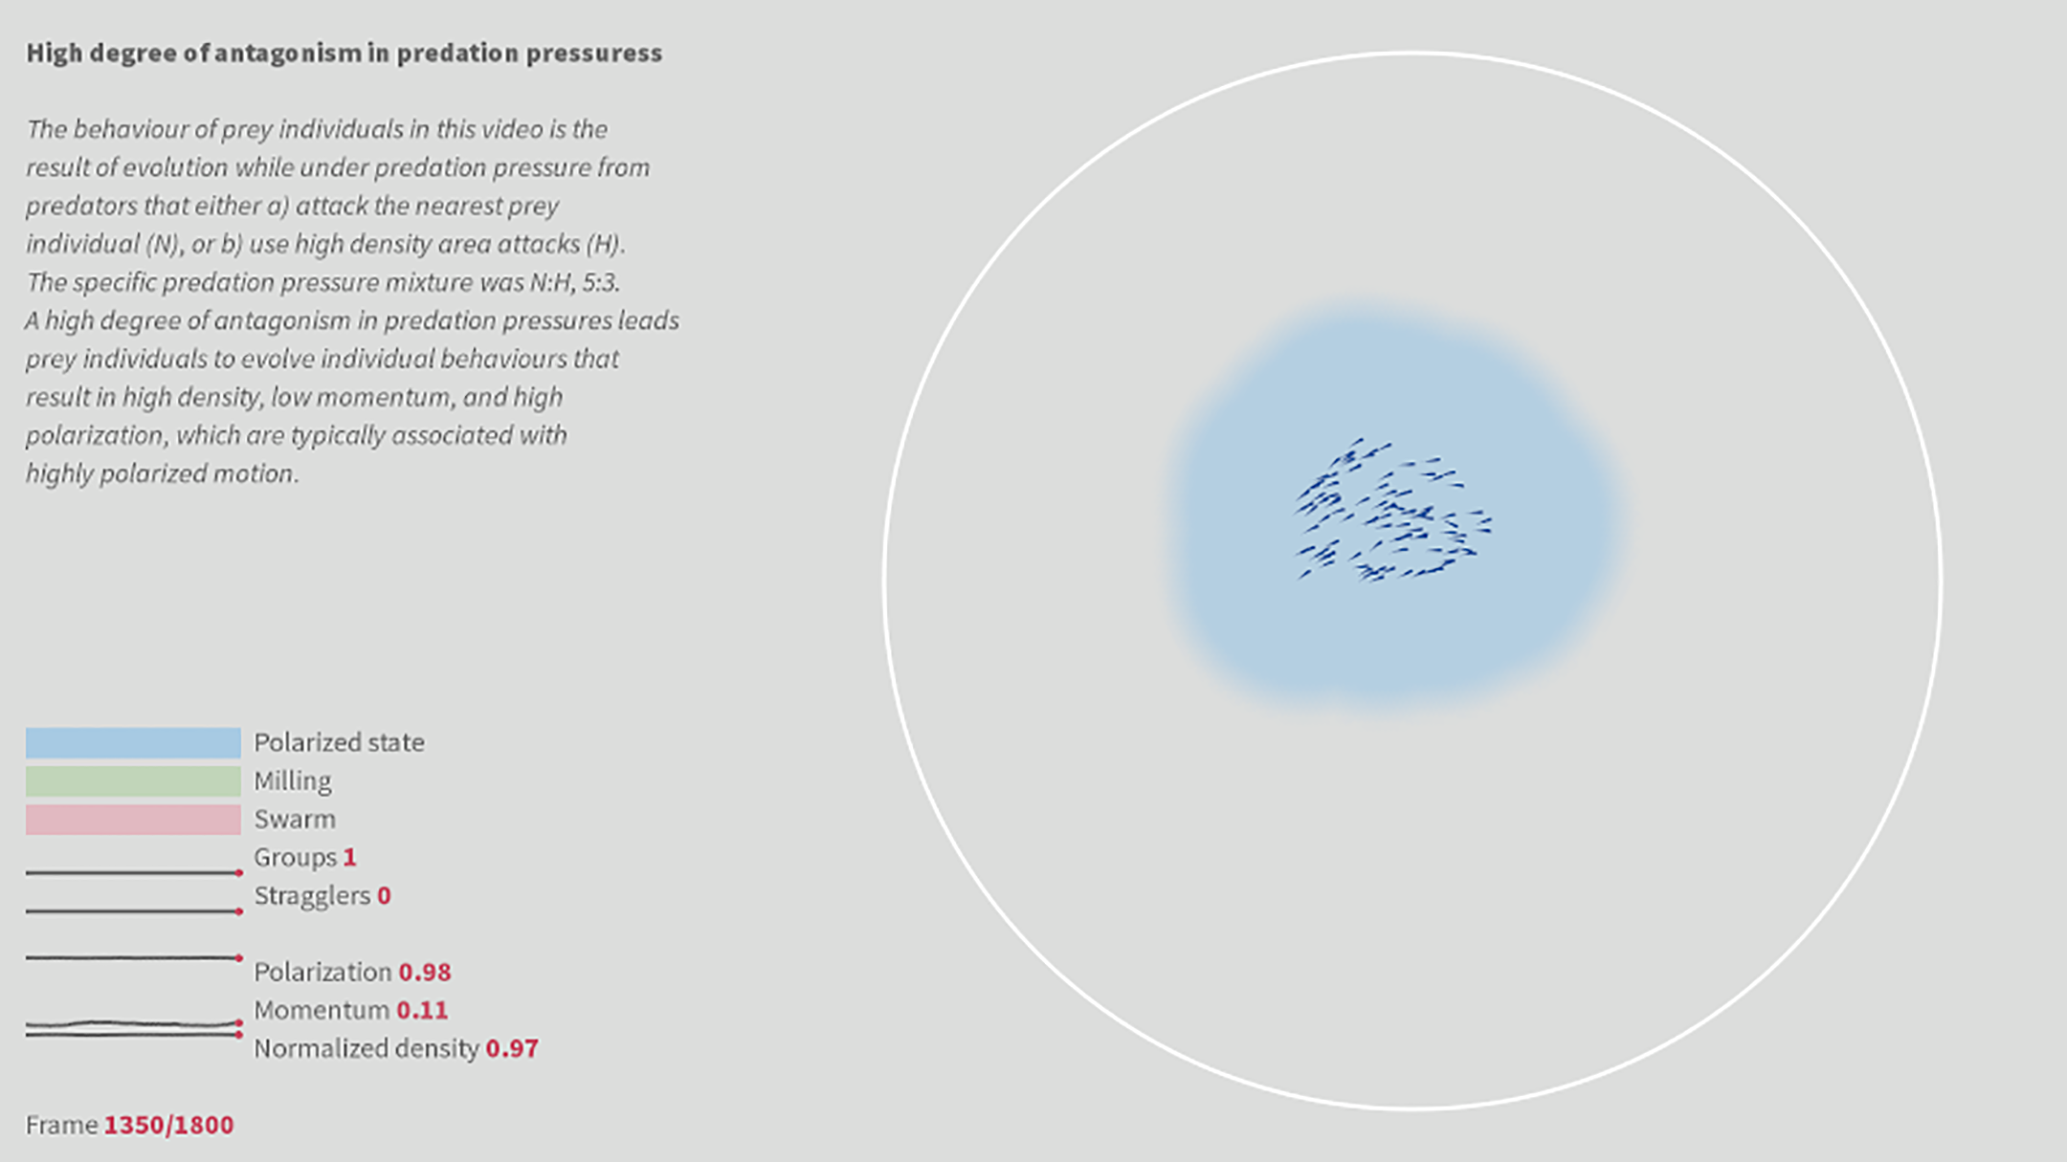
\includegraphics[width=\figurewidth]{scirep/si-V7_1350}
  \infigurecaption{The behaviour of prey individuals in this video is the result of evolution while under predation pressure from predators that either a) attack the nearest prey individual (N), or b) use high density area attacks (H). The specific predation pressure mixture was N:H, 5:3. A high degree of antagonism in predation pressures leads prey individuals to evolve individual behaviours that result in high density, low momentum, and high polarization, which are typically associated with highly polarized motion.}
  \caption{High degree of antagonism in predation pressures.}
  \label{video:V7}
\end{video}

 % include suplementary material

\end{subappendices}
